% Seminarul 3: Rădăcini unitare și modele ARIMA
% Serii de timp -- Programele de licență Informatică economică și Cibernetică economică, Academia de Studii Economice din București
% GENERAT de latex/build_seminar3.py -- modificați generatorul, nu acest fișier.
% Implicit versiunea pentru studenți; versiunea profesorului este wrapper-ul *_solutions.tex.
\makeatletter\@ifundefined{ifsolutions}{\expandafter\newif\csname ifsolutions\endcsname}{}\makeatother

\newcommand{\coursename}{Serii de timp}
\def\tsalang{ro}
% Preambul comun TSA -- Serii de timp / Time Series Analysis (Beamer, 16:9)
% Același design ca MFM și SFM (preluat din SFM, 5 octombrie 2026). Înainte de % Preambul comun TSA -- Serii de timp / Time Series Analysis (Beamer, 16:9)
% Același design ca MFM și SFM (preluat din SFM, 5 octombrie 2026). Înainte de % Preambul comun TSA -- Serii de timp / Time Series Analysis (Beamer, 16:9)
% Același design ca MFM și SFM (preluat din SFM, 5 octombrie 2026). Înainte de \input{../../latex/preamble} se definește
%   \newcommand{\coursename}{Time Series Analysis}      (EN)
%   \newcommand{\coursename}{Serii de timp}       (RO)  și  \def\tsalang{ro}
% Fișierele .tex se află în EN/Courses, EN/Seminars, RO/Cursuri, RO/Seminarii (două niveluri sub rădăcină).
% Deck-urile sînt generate de latex/build_chapterN.py / build_seminarN.py (vezi latex/tsa_build.py).

\documentclass[9pt, aspectratio=169, t]{beamer}
\providecommand{\coursename}{Time Series Analysis}

% Ensure content fits on slides
\setbeamersize{text margin left=8mm, text margin right=8mm}
% Smaller institute font (title page)
\setbeamerfont{institute}{size=\footnotesize}

%=============================================================================
% THEME AND STYLE CONFIGURATION
%=============================================================================
\usetheme{default}
% Using default theme for clean header/footer control

% Color Palette (matching Redispatch PDF)
\definecolor{MainBlue}{RGB}{26, 58, 110}
\definecolor{AccentBlue}{RGB}{26, 58, 110}
\definecolor{IDAred}{RGB}{205, 0, 0}
\definecolor{DarkGray}{RGB}{51, 51, 51}
\definecolor{MediumGray}{RGB}{128, 128, 128}
\definecolor{LightGray}{RGB}{248, 248, 248}
\definecolor{VeryLightGray}{RGB}{235, 235, 235}
\definecolor{KeynoteGray}{RGB}{218, 218, 218}
\definecolor{SectionGray}{RGB}{120, 120, 120}
\definecolor{FooterGray}{RGB}{100, 100, 100}
\definecolor{Crimson}{RGB}{220, 53, 69}
\definecolor{Forest}{RGB}{46, 125, 50}
\definecolor{Amber}{RGB}{181, 133, 63}
\definecolor{Orange}{RGB}{230, 126, 34}
\definecolor{Purple}{RGB}{142, 68, 173}

% Gradient background (exact Keynote 315° gradient: white to RGB 218,218,218)
\setbeamertemplate{background}{%
    \begin{tikzpicture}[remember picture, overlay]
        \shade[shading=axis, shading angle=315,
        top color=white, bottom color=KeynoteGray]
        (current page.south west) rectangle (current page.north east);
    \end{tikzpicture}%
}
% Fallback solid color for compatibility
\setbeamercolor{background canvas}{bg=}

\setbeamercolor{palette primary}{bg=MainBlue, fg=white}
\setbeamercolor{palette secondary}{bg=MainBlue!85, fg=white}
\setbeamercolor{palette tertiary}{bg=MainBlue!70, fg=white}
\setbeamercolor{structure}{fg=MainBlue}
\setbeamercolor{title}{fg=IDAred}
\setbeamercolor{frametitle}{fg=IDAred, bg=}
\setbeamercolor{block title}{bg=MainBlue, fg=white}
\setbeamercolor{block body}{bg=VeryLightGray, fg=DarkGray}
\setbeamercolor{block title alerted}{bg=Crimson, fg=white}
\setbeamercolor{block body alerted}{bg=Crimson!8, fg=DarkGray}
\setbeamercolor{block title example}{bg=Forest, fg=white}
\setbeamercolor{block body example}{bg=Forest!8, fg=DarkGray}
\setbeamercolor{item}{fg=MainBlue}

% Footer colors (override Madrid theme blue)
\setbeamercolor{author in head/foot}{fg=FooterGray, bg=}
\setbeamercolor{title in head/foot}{fg=FooterGray, bg=}
\setbeamercolor{date in head/foot}{fg=FooterGray, bg=}
\setbeamercolor{section in head/foot}{fg=FooterGray, bg=}
\setbeamercolor{subsection in head/foot}{fg=FooterGray, bg=}

% Bullet styles (apply everywhere including blocks)
\setbeamertemplate{itemize item}{\color{MainBlue}$\boxdot$}
\setbeamertemplate{itemize subitem}{\color{MainBlue}$\blacktriangleright$}
\setbeamertemplate{itemize subsubitem}{\color{MainBlue}\tiny$\bullet$}
\setbeamertemplate{itemize/enumerate body begin}{\normalsize}
\setbeamertemplate{itemize/enumerate subbody begin}{\normalsize}

% Item spacing - compact style
\setlength{\leftmargini}{10pt}       % Level 1: minimal indent
\setlength{\leftmarginii}{10pt}      % Level 2: minimal additional indent
% Compact list spacing (zero extra space before/after lists in blocks)
\makeatletter
\def\@listi{\leftmargin\leftmargini \topsep 0pt \parsep 0pt \itemsep 0pt}
\def\@listii{\leftmargin\leftmarginii \topsep 0pt \parsep 0pt \itemsep 0pt}
\makeatother

\setbeamertemplate{navigation symbols}{}

%=============================================================================
% CUSTOM HEADLINE
%=============================================================================
\setbeamertemplate{headline}{%
    \vskip10pt%
    \hbox to \paperwidth{%
        \hskip0.5cm%
        {\small\color{FooterGray}\renewcommand{\hyperlink}[2]{##2}\insertsectionhead}%
        \hfill%
        \textcolor{FooterGray}{\small\insertframenumber}%
        \hskip0.5cm%
    }%
    \vskip4pt%
    {\color{FooterGray}\hrule height 0.4pt}%
}

%=============================================================================
% CUSTOM FOOTER
%=============================================================================
\usepackage{fontawesome5}

\setbeamertemplate{footline}{%
    {\color{FooterGray}\hrule height 0.4pt}%
    \vskip4pt%
    \hbox to \paperwidth{%
        \hskip0.5cm%
        \textcolor{FooterGray}{\small\coursename}%
        \hfill%
        \raisebox{-0.1em}{%
            \begin{tikzpicture}[x=0.08em, y=0.08em, line width=0.4pt]
                \draw[FooterGray] (0,3) -- (1,4) -- (2,3.5) -- (3,5) -- (4,4) -- (5,6) -- (6,5.5) -- (7,4) -- (8,5) -- (9,7) -- (10,6) -- (11,5) -- (12,6.5) -- (13,8) -- (14,7) -- (15,6) -- (16,7.5) -- (17,9) -- (18,8) -- (19,7) -- (20,8.5) -- (21,10) -- (22,9) -- (23,8) -- (24,9.5);
            \end{tikzpicture}%
        }%
        \hskip0.5cm%
    }%
    \vskip6pt%
}

%=============================================================================
% PACKAGES
%=============================================================================
\usepackage[utf8]{inputenc}
\DeclareUnicodeCharacter{03B1}{\ensuremath{\alpha}}
\usepackage[T1]{fontenc}
\usepackage{amsmath, amssymb, amsthm}
\usepackage{mathtools}
\usepackage{bm}
\usepackage{tikz}
\usetikzlibrary{arrows.meta, positioning, shapes, calc, decorations.pathreplacing, shadings}
\usepackage{booktabs}
\usepackage{multirow}
\usepackage{array}
\usepackage{graphicx}
\usepackage{animate}
\usepackage{hyperref}
\usepackage{colortbl}
\usepackage{listings}
\lstset{language=Python, basicstyle=\ttfamily\scriptsize, keywordstyle=\color{MainBlue}\bfseries,
  commentstyle=\color{Forest}, stringstyle=\color{Crimson}, breaklines=true,
  frame=none, backgroundcolor=\color{VeryLightGray}, xleftmargin=2mm}
\hypersetup{colorlinks=true, linkcolor=MainBlue, urlcolor=MainBlue}
\graphicspath{{../../logos/}{../../charts/}{../../photos/}}
\usepackage{xcolor}
\hfuzz=2pt  % Suppress tiny overfull warnings (<2pt)
\vfuzz=2pt  % Suppress tiny vertical overfull warnings (<2pt)
% \mathrm in the sans-serif family of the slides (beamer resets \mathrm to the serif family at \begin{document};
% this hook runs after beamer's, so WN, Var, RMSE, ... in formulas match the surrounding text)
% Bold vectors and matrices in the same sans-serif family: \mathbf{A} in sans bold (beamer's own \mathbf came out in
% medium weight), and the bold upright Greek capitals of \boldsymbol / \bm (\bSigma, \bPhi, \boldsymbol{\Theta}) in
% cmss bold: bm.sty fixes its "boldoperators" font when it is loaded (serif cmbx), before beamer switches the
% operators to cmss, so it is reset here.
\AtBeginDocument{%
  \SetMathAlphabet{\mathrm}{normal}{\encodingdefault}{\sfdefault}{\mddefault}{n}%
  \SetMathAlphabet{\mathrm}{bold}{\encodingdefault}{\sfdefault}{bx}{n}%
  \SetMathAlphabet{\mathbf}{normal}{\encodingdefault}{\sfdefault}{bx}{n}%
  \SetMathAlphabet{\mathbf}{bold}{\encodingdefault}{\sfdefault}{bx}{n}%
  \SetSymbolFont{boldoperators}{normal}{OT1}{cmss}{bx}{n}%
  \SetSymbolFont{boldoperators}{bold}{OT1}{cmss}{bx}{n}}

%=============================================================================
% QUANTLET COMMANDS
%   \quantlet{<displayed name>}{<url>}       (generic, compatible with the older TSA decks)
%   \tsaquantlet{Ch_05}{TSA_ch5_garch}       -> https://github.com/danpele/Time-Series-Analysis/tree/main/Quantlets/Ch_05/TSA_ch5_garch
%   \qlurl{<folder>} is defined per chapter by the generator (Quantlets/Ch_NN/<folder>)
%=============================================================================
\newcommand{\tsarepo}{https://github.com/danpele/Time-Series-Analysis}
\newcommand{\tsaqlbase}{https://github.com/danpele/Time-Series-Analysis/tree/main/Quantlets}
\newcommand{\quantlet}[2]{%
    \hfill\href{#2}{%
        \raisebox{-0.15em}{
\includegraphics[height=0.7em]{ql_logo.png}}%
        \textcolor{MainBlue}{\tiny\ #1}%
    }%
}
\newcommand{\tsaquantlet}[2]{\quantlet{\detokenize{#2}}{\tsaqlbase/#1/#2}}

%=============================================================================
% NOTEBOOKS (Google Colab)
%   \colaburl{notebooks/EN/chapter5_seminar_notebook.ipynb} -> the Colab link of a file in the TSA repo
%   \nb: the chapter notebook (each seminar deck redefines it with \renewcommand)
%=============================================================================
\newcommand{\colaburl}[1]{https://colab.research.google.com/github/danpele/Time-Series-Analysis/blob/main/#1}
\newcommand{\nb}{https://colab.research.google.com/github/danpele/Time-Series-Analysis/tree/main/notebooks/EN}
\newcommand{\nbname}{notebooks/EN}

%=============================================================================
% SLIDE HELPERS (used by the generators; the same as in MFM)
%=============================================================================
% local font size for list bodies (the preamble forces \normalsize)
\newcommand{\itemsize}[1]{\setbeamertemplate{itemize/enumerate body begin}{#1}\setbeamertemplate{itemize/enumerate subbody begin}{#1}}
\newcommand{\intitle}[1]{{\hypersetup{urlcolor=white}#1}}   % white links inside coloured title bars
\newcommand{\imgcap}[1]{{\scriptsize #1}\\[0.5mm]}          % caption under a photo
\newcommand{\imgcredit}[2]{{\tiny\color{FooterGray}\href{#1}{#2}}}   % image credit: source URL, author/licence
\newcommand{\aiprompt}[1]{{\ttfamily\color{MainBlue}#1}}     % a prompt to an AI assistant

%=============================================================================
% SEMINARS: student version by default; the instructor wrapper *_solutions.tex sets \solutionstrue
%=============================================================================
\makeatletter\@ifundefined{ifsolutions}{\expandafter\newif\csname ifsolutions\endcsname}{}\makeatother
\newcommand{\solonly}[1]{\ifsolutions #1\fi}
\newcommand{\propsub}{\ifsolutions\else\framesubtitle{\ifdefined\tsalang Rezolvarea se discută la seminar\else Solution discussed in class\fi}\fi}

%=============================================================================
% APPENDIX AND CHAPTER LINKS (latex/appendix_links.py writes the calls; it also re-declares these
% macros before \begin{document}, so the decks compile with or without this preamble block)
%=============================================================================
\providecommand{\tsaapplink}[3]{\hypertarget{#2}{}\hyperlink{#1}{\beamergotobutton{#3}}}
\providecommand{\tsaappback}[2]{\begin{tikzpicture}[remember picture,overlay]\node[anchor=south east] at ([xshift=-3mm,yshift=7mm]current page.south east){\hyperlink{#1}{\beamerreturnbutton{#2}}};\end{tikzpicture}}
\providecommand{\tsachlink}[2]{\href{#1}{#2}}
\providecommand{\tsachlinkt}[2]{\href{#1}{\usebeamercolor[fg]{frametitle}#2}}

%=============================================================================
% QUANTINAR COMMAND: link către un curs Quantinar (subiecte avansate)
%=============================================================================
\newcommand{\quantinar}[2]{%
    \href{#2}{%
        \raisebox{-0.15em}{
\includegraphics[height=0.8em]{qr_logo.png}}%
        \textcolor{MainBlue}{\scriptsize\ #1}%
    }%
}

%=============================================================================
% CUSTOM TITLE PAGE
%=============================================================================
\defbeamertemplate*{title page}{hybrid}[1][]
{
    \vspace{0.2cm}
    % Logos row - top header (with clickable links)
    \begin{center}
        \href{https://www.ase.ro}{
\includegraphics[height=1.0cm]{ase_logo.png}}\hspace{0.3cm}%
        \href{https://theida.net}{
\includegraphics[height=1.0cm]{ida_logo.png}}\hspace{0.3cm}%
        \href{https://blockchain-research-center.com}{
\includegraphics[height=1.0cm]{brc_logo.png}}\hspace{0.3cm}%
        \href{https://www.ai4efin.ase.ro}{
\includegraphics[height=1.0cm]{ai4efin_logo.png}}\hspace{0.3cm}%
        \href{https://ipe.ro/new}{
\includegraphics[height=1.0cm]{acad_logo.png}}\hspace{0.3cm}%
        \href{https://www.digital-finance-msca.com}{
\includegraphics[height=1.0cm]{msca_logo.png}}%
    \end{center}

    \vspace{0.6cm}

    % Main title with Q logos on sides (with clickable links)
    \begin{center}
        \begin{minipage}{0.1\textwidth}
            \centering
            \href{https://quantlet.com}{
\includegraphics[height=1.1cm]{ql_logo.png}}
        \end{minipage}%
        \begin{minipage}{0.78\textwidth}
            \centering
            {\LARGE\bfseries\usebeamercolor[fg]{title}\inserttitle}

            \vspace{0.3cm}

            {\usebeamerfont{subtitle}\usebeamercolor[fg]{title}\insertsubtitle}
        \end{minipage}%
        \begin{minipage}{0.1\textwidth}
            \centering
            \href{https://quantinar.com}{
\includegraphics[height=1.1cm]{qr_logo.png}}
        \end{minipage}
    \end{center}

    \vspace{0.6cm}

    % Authors (left aligned)
    \hspace{0.5cm}{\usebeamerfont{author}\insertauthor}

    \vspace{0.3cm}

    % Institute/Affiliations (left aligned)
    \hspace{0.5cm}\begin{minipage}[t]{0.9\textwidth}
        \raggedright\small\insertinstitute
    \end{minipage}
}

%=============================================================================
% THEOREM ENVIRONMENTS
%=============================================================================
\theoremstyle{definition}
\setbeamertemplate{theorems}[numbered]
\ifdefined\tsalang
\newtheorem{defn}{Definiție}
\newtheorem{thm}{Teoremă}
\newtheorem{prop}{Propoziție}
\newtheorem{rmk}{Observație}
\else
\newtheorem{defn}{Definition}
\newtheorem{thm}{Theorem}
\newtheorem{prop}{Proposition}
\newtheorem{rmk}{Remark}
\fi

%=============================================================================
% CENTRED MINIPAGE (no extra vertical space)
%=============================================================================
\newenvironment{cminipage}[1]{%
    \par\noindent\hfill\begin{minipage}{#1}\ignorespaces
}{%
    \end{minipage}\hfill\null\par
}

%=============================================================================
% CUSTOM COMMANDS
%=============================================================================
\newcommand{\E}{\mathbb{E}}
\newcommand{\Var}{\text{Var}}
\newcommand{\Cov}{\text{Cov}}
\newcommand{\Corr}{\text{Corr}}
\newcommand{\R}{\mathbb{R}}
\newcommand{\N}{\mathbb{N}}
\newcommand{\Z}{\mathbb{Z}}
\newcommand{\B}{\mathbf{B}}
\newcommand{\imark}{\textcolor{MainBlue}{\textbullet}}
\newcommand{\RMSE}{\text{RMSE}}
\newcommand{\MAE}{\text{MAE}}
\newcommand{\MAPE}{\text{MAPE}}

% Boldface vector/matrix commands (VAR, VECM, state space; also used by the older TSA decks)
\newcommand{\bY}{\mathbf{Y}}
\newcommand{\bX}{\mathbf{X}}
\newcommand{\bA}{\mathbf{A}}
\newcommand{\bB}{\mathbf{B}}
\newcommand{\bepsilon}{\boldsymbol{\varepsilon}}
\newcommand{\bSigma}{\boldsymbol{\Sigma}}
\newcommand{\bPhi}{\boldsymbol{\Phi}}
\newcommand{\bGamma}{\boldsymbol{\Gamma}}
\newcommand{\bPi}{\boldsymbol{\Pi}}
\newcommand{\bc}{\mathbf{c}}
\newcommand{\balpha}{\boldsymbol{\alpha}}
\newcommand{\bbeta}{\boldsymbol{\beta}}
\newcommand{\bvarepsilon}{\boldsymbol{\varepsilon}}

% Legacy seminar marks (older TSA seminar decks)
\newcommand{\correct}{\textcolor{Forest}{\checkmark}}
\newcommand{\incorrect}{\textcolor{Crimson}{\texttimes}}
 se definește
%   \newcommand{\coursename}{Time Series Analysis}      (EN)
%   \newcommand{\coursename}{Serii de timp}       (RO)  și  \def\tsalang{ro}
% Fișierele .tex se află în EN/Courses, EN/Seminars, RO/Cursuri, RO/Seminarii (două niveluri sub rădăcină).
% Deck-urile sînt generate de latex/build_chapterN.py / build_seminarN.py (vezi latex/tsa_build.py).

\documentclass[9pt, aspectratio=169, t]{beamer}
\providecommand{\coursename}{Time Series Analysis}

% Ensure content fits on slides
\setbeamersize{text margin left=8mm, text margin right=8mm}
% Smaller institute font (title page)
\setbeamerfont{institute}{size=\footnotesize}

%=============================================================================
% THEME AND STYLE CONFIGURATION
%=============================================================================
\usetheme{default}
% Using default theme for clean header/footer control

% Color Palette (matching Redispatch PDF)
\definecolor{MainBlue}{RGB}{26, 58, 110}
\definecolor{AccentBlue}{RGB}{26, 58, 110}
\definecolor{IDAred}{RGB}{205, 0, 0}
\definecolor{DarkGray}{RGB}{51, 51, 51}
\definecolor{MediumGray}{RGB}{128, 128, 128}
\definecolor{LightGray}{RGB}{248, 248, 248}
\definecolor{VeryLightGray}{RGB}{235, 235, 235}
\definecolor{KeynoteGray}{RGB}{218, 218, 218}
\definecolor{SectionGray}{RGB}{120, 120, 120}
\definecolor{FooterGray}{RGB}{100, 100, 100}
\definecolor{Crimson}{RGB}{220, 53, 69}
\definecolor{Forest}{RGB}{46, 125, 50}
\definecolor{Amber}{RGB}{181, 133, 63}
\definecolor{Orange}{RGB}{230, 126, 34}
\definecolor{Purple}{RGB}{142, 68, 173}

% Gradient background (exact Keynote 315° gradient: white to RGB 218,218,218)
\setbeamertemplate{background}{%
    \begin{tikzpicture}[remember picture, overlay]
        \shade[shading=axis, shading angle=315,
        top color=white, bottom color=KeynoteGray]
        (current page.south west) rectangle (current page.north east);
    \end{tikzpicture}%
}
% Fallback solid color for compatibility
\setbeamercolor{background canvas}{bg=}

\setbeamercolor{palette primary}{bg=MainBlue, fg=white}
\setbeamercolor{palette secondary}{bg=MainBlue!85, fg=white}
\setbeamercolor{palette tertiary}{bg=MainBlue!70, fg=white}
\setbeamercolor{structure}{fg=MainBlue}
\setbeamercolor{title}{fg=IDAred}
\setbeamercolor{frametitle}{fg=IDAred, bg=}
\setbeamercolor{block title}{bg=MainBlue, fg=white}
\setbeamercolor{block body}{bg=VeryLightGray, fg=DarkGray}
\setbeamercolor{block title alerted}{bg=Crimson, fg=white}
\setbeamercolor{block body alerted}{bg=Crimson!8, fg=DarkGray}
\setbeamercolor{block title example}{bg=Forest, fg=white}
\setbeamercolor{block body example}{bg=Forest!8, fg=DarkGray}
\setbeamercolor{item}{fg=MainBlue}

% Footer colors (override Madrid theme blue)
\setbeamercolor{author in head/foot}{fg=FooterGray, bg=}
\setbeamercolor{title in head/foot}{fg=FooterGray, bg=}
\setbeamercolor{date in head/foot}{fg=FooterGray, bg=}
\setbeamercolor{section in head/foot}{fg=FooterGray, bg=}
\setbeamercolor{subsection in head/foot}{fg=FooterGray, bg=}

% Bullet styles (apply everywhere including blocks)
\setbeamertemplate{itemize item}{\color{MainBlue}$\boxdot$}
\setbeamertemplate{itemize subitem}{\color{MainBlue}$\blacktriangleright$}
\setbeamertemplate{itemize subsubitem}{\color{MainBlue}\tiny$\bullet$}
\setbeamertemplate{itemize/enumerate body begin}{\normalsize}
\setbeamertemplate{itemize/enumerate subbody begin}{\normalsize}

% Item spacing - compact style
\setlength{\leftmargini}{10pt}       % Level 1: minimal indent
\setlength{\leftmarginii}{10pt}      % Level 2: minimal additional indent
% Compact list spacing (zero extra space before/after lists in blocks)
\makeatletter
\def\@listi{\leftmargin\leftmargini \topsep 0pt \parsep 0pt \itemsep 0pt}
\def\@listii{\leftmargin\leftmarginii \topsep 0pt \parsep 0pt \itemsep 0pt}
\makeatother

\setbeamertemplate{navigation symbols}{}

%=============================================================================
% CUSTOM HEADLINE
%=============================================================================
\setbeamertemplate{headline}{%
    \vskip10pt%
    \hbox to \paperwidth{%
        \hskip0.5cm%
        {\small\color{FooterGray}\renewcommand{\hyperlink}[2]{##2}\insertsectionhead}%
        \hfill%
        \textcolor{FooterGray}{\small\insertframenumber}%
        \hskip0.5cm%
    }%
    \vskip4pt%
    {\color{FooterGray}\hrule height 0.4pt}%
}

%=============================================================================
% CUSTOM FOOTER
%=============================================================================
\usepackage{fontawesome5}

\setbeamertemplate{footline}{%
    {\color{FooterGray}\hrule height 0.4pt}%
    \vskip4pt%
    \hbox to \paperwidth{%
        \hskip0.5cm%
        \textcolor{FooterGray}{\small\coursename}%
        \hfill%
        \raisebox{-0.1em}{%
            \begin{tikzpicture}[x=0.08em, y=0.08em, line width=0.4pt]
                \draw[FooterGray] (0,3) -- (1,4) -- (2,3.5) -- (3,5) -- (4,4) -- (5,6) -- (6,5.5) -- (7,4) -- (8,5) -- (9,7) -- (10,6) -- (11,5) -- (12,6.5) -- (13,8) -- (14,7) -- (15,6) -- (16,7.5) -- (17,9) -- (18,8) -- (19,7) -- (20,8.5) -- (21,10) -- (22,9) -- (23,8) -- (24,9.5);
            \end{tikzpicture}%
        }%
        \hskip0.5cm%
    }%
    \vskip6pt%
}

%=============================================================================
% PACKAGES
%=============================================================================
\usepackage[utf8]{inputenc}
\DeclareUnicodeCharacter{03B1}{\ensuremath{\alpha}}
\usepackage[T1]{fontenc}
\usepackage{amsmath, amssymb, amsthm}
\usepackage{mathtools}
\usepackage{bm}
\usepackage{tikz}
\usetikzlibrary{arrows.meta, positioning, shapes, calc, decorations.pathreplacing, shadings}
\usepackage{booktabs}
\usepackage{multirow}
\usepackage{array}
\usepackage{graphicx}
\usepackage{animate}
\usepackage{hyperref}
\usepackage{colortbl}
\usepackage{listings}
\lstset{language=Python, basicstyle=\ttfamily\scriptsize, keywordstyle=\color{MainBlue}\bfseries,
  commentstyle=\color{Forest}, stringstyle=\color{Crimson}, breaklines=true,
  frame=none, backgroundcolor=\color{VeryLightGray}, xleftmargin=2mm}
\hypersetup{colorlinks=true, linkcolor=MainBlue, urlcolor=MainBlue}
\graphicspath{{../../logos/}{../../charts/}{../../photos/}}
\usepackage{xcolor}
\hfuzz=2pt  % Suppress tiny overfull warnings (<2pt)
\vfuzz=2pt  % Suppress tiny vertical overfull warnings (<2pt)
% \mathrm in the sans-serif family of the slides (beamer resets \mathrm to the serif family at \begin{document};
% this hook runs after beamer's, so WN, Var, RMSE, ... in formulas match the surrounding text)
% Bold vectors and matrices in the same sans-serif family: \mathbf{A} in sans bold (beamer's own \mathbf came out in
% medium weight), and the bold upright Greek capitals of \boldsymbol / \bm (\bSigma, \bPhi, \boldsymbol{\Theta}) in
% cmss bold: bm.sty fixes its "boldoperators" font when it is loaded (serif cmbx), before beamer switches the
% operators to cmss, so it is reset here.
\AtBeginDocument{%
  \SetMathAlphabet{\mathrm}{normal}{\encodingdefault}{\sfdefault}{\mddefault}{n}%
  \SetMathAlphabet{\mathrm}{bold}{\encodingdefault}{\sfdefault}{bx}{n}%
  \SetMathAlphabet{\mathbf}{normal}{\encodingdefault}{\sfdefault}{bx}{n}%
  \SetMathAlphabet{\mathbf}{bold}{\encodingdefault}{\sfdefault}{bx}{n}%
  \SetSymbolFont{boldoperators}{normal}{OT1}{cmss}{bx}{n}%
  \SetSymbolFont{boldoperators}{bold}{OT1}{cmss}{bx}{n}}

%=============================================================================
% QUANTLET COMMANDS
%   \quantlet{<displayed name>}{<url>}       (generic, compatible with the older TSA decks)
%   \tsaquantlet{Ch_05}{TSA_ch5_garch}       -> https://github.com/danpele/Time-Series-Analysis/tree/main/Quantlets/Ch_05/TSA_ch5_garch
%   \qlurl{<folder>} is defined per chapter by the generator (Quantlets/Ch_NN/<folder>)
%=============================================================================
\newcommand{\tsarepo}{https://github.com/danpele/Time-Series-Analysis}
\newcommand{\tsaqlbase}{https://github.com/danpele/Time-Series-Analysis/tree/main/Quantlets}
\newcommand{\quantlet}[2]{%
    \hfill\href{#2}{%
        \raisebox{-0.15em}{
\includegraphics[height=0.7em]{ql_logo.png}}%
        \textcolor{MainBlue}{\tiny\ #1}%
    }%
}
\newcommand{\tsaquantlet}[2]{\quantlet{\detokenize{#2}}{\tsaqlbase/#1/#2}}

%=============================================================================
% NOTEBOOKS (Google Colab)
%   \colaburl{notebooks/EN/chapter5_seminar_notebook.ipynb} -> the Colab link of a file in the TSA repo
%   \nb: the chapter notebook (each seminar deck redefines it with \renewcommand)
%=============================================================================
\newcommand{\colaburl}[1]{https://colab.research.google.com/github/danpele/Time-Series-Analysis/blob/main/#1}
\newcommand{\nb}{https://colab.research.google.com/github/danpele/Time-Series-Analysis/tree/main/notebooks/EN}
\newcommand{\nbname}{notebooks/EN}

%=============================================================================
% SLIDE HELPERS (used by the generators; the same as in MFM)
%=============================================================================
% local font size for list bodies (the preamble forces \normalsize)
\newcommand{\itemsize}[1]{\setbeamertemplate{itemize/enumerate body begin}{#1}\setbeamertemplate{itemize/enumerate subbody begin}{#1}}
\newcommand{\intitle}[1]{{\hypersetup{urlcolor=white}#1}}   % white links inside coloured title bars
\newcommand{\imgcap}[1]{{\scriptsize #1}\\[0.5mm]}          % caption under a photo
\newcommand{\imgcredit}[2]{{\tiny\color{FooterGray}\href{#1}{#2}}}   % image credit: source URL, author/licence
\newcommand{\aiprompt}[1]{{\ttfamily\color{MainBlue}#1}}     % a prompt to an AI assistant

%=============================================================================
% SEMINARS: student version by default; the instructor wrapper *_solutions.tex sets \solutionstrue
%=============================================================================
\makeatletter\@ifundefined{ifsolutions}{\expandafter\newif\csname ifsolutions\endcsname}{}\makeatother
\newcommand{\solonly}[1]{\ifsolutions #1\fi}
\newcommand{\propsub}{\ifsolutions\else\framesubtitle{\ifdefined\tsalang Rezolvarea se discută la seminar\else Solution discussed in class\fi}\fi}

%=============================================================================
% APPENDIX AND CHAPTER LINKS (latex/appendix_links.py writes the calls; it also re-declares these
% macros before \begin{document}, so the decks compile with or without this preamble block)
%=============================================================================
\providecommand{\tsaapplink}[3]{\hypertarget{#2}{}\hyperlink{#1}{\beamergotobutton{#3}}}
\providecommand{\tsaappback}[2]{\begin{tikzpicture}[remember picture,overlay]\node[anchor=south east] at ([xshift=-3mm,yshift=7mm]current page.south east){\hyperlink{#1}{\beamerreturnbutton{#2}}};\end{tikzpicture}}
\providecommand{\tsachlink}[2]{\href{#1}{#2}}
\providecommand{\tsachlinkt}[2]{\href{#1}{\usebeamercolor[fg]{frametitle}#2}}

%=============================================================================
% QUANTINAR COMMAND: link către un curs Quantinar (subiecte avansate)
%=============================================================================
\newcommand{\quantinar}[2]{%
    \href{#2}{%
        \raisebox{-0.15em}{
\includegraphics[height=0.8em]{qr_logo.png}}%
        \textcolor{MainBlue}{\scriptsize\ #1}%
    }%
}

%=============================================================================
% CUSTOM TITLE PAGE
%=============================================================================
\defbeamertemplate*{title page}{hybrid}[1][]
{
    \vspace{0.2cm}
    % Logos row - top header (with clickable links)
    \begin{center}
        \href{https://www.ase.ro}{
\includegraphics[height=1.0cm]{ase_logo.png}}\hspace{0.3cm}%
        \href{https://theida.net}{
\includegraphics[height=1.0cm]{ida_logo.png}}\hspace{0.3cm}%
        \href{https://blockchain-research-center.com}{
\includegraphics[height=1.0cm]{brc_logo.png}}\hspace{0.3cm}%
        \href{https://www.ai4efin.ase.ro}{
\includegraphics[height=1.0cm]{ai4efin_logo.png}}\hspace{0.3cm}%
        \href{https://ipe.ro/new}{
\includegraphics[height=1.0cm]{acad_logo.png}}\hspace{0.3cm}%
        \href{https://www.digital-finance-msca.com}{
\includegraphics[height=1.0cm]{msca_logo.png}}%
    \end{center}

    \vspace{0.6cm}

    % Main title with Q logos on sides (with clickable links)
    \begin{center}
        \begin{minipage}{0.1\textwidth}
            \centering
            \href{https://quantlet.com}{
\includegraphics[height=1.1cm]{ql_logo.png}}
        \end{minipage}%
        \begin{minipage}{0.78\textwidth}
            \centering
            {\LARGE\bfseries\usebeamercolor[fg]{title}\inserttitle}

            \vspace{0.3cm}

            {\usebeamerfont{subtitle}\usebeamercolor[fg]{title}\insertsubtitle}
        \end{minipage}%
        \begin{minipage}{0.1\textwidth}
            \centering
            \href{https://quantinar.com}{
\includegraphics[height=1.1cm]{qr_logo.png}}
        \end{minipage}
    \end{center}

    \vspace{0.6cm}

    % Authors (left aligned)
    \hspace{0.5cm}{\usebeamerfont{author}\insertauthor}

    \vspace{0.3cm}

    % Institute/Affiliations (left aligned)
    \hspace{0.5cm}\begin{minipage}[t]{0.9\textwidth}
        \raggedright\small\insertinstitute
    \end{minipage}
}

%=============================================================================
% THEOREM ENVIRONMENTS
%=============================================================================
\theoremstyle{definition}
\setbeamertemplate{theorems}[numbered]
\ifdefined\tsalang
\newtheorem{defn}{Definiție}
\newtheorem{thm}{Teoremă}
\newtheorem{prop}{Propoziție}
\newtheorem{rmk}{Observație}
\else
\newtheorem{defn}{Definition}
\newtheorem{thm}{Theorem}
\newtheorem{prop}{Proposition}
\newtheorem{rmk}{Remark}
\fi

%=============================================================================
% CENTRED MINIPAGE (no extra vertical space)
%=============================================================================
\newenvironment{cminipage}[1]{%
    \par\noindent\hfill\begin{minipage}{#1}\ignorespaces
}{%
    \end{minipage}\hfill\null\par
}

%=============================================================================
% CUSTOM COMMANDS
%=============================================================================
\newcommand{\E}{\mathbb{E}}
\newcommand{\Var}{\text{Var}}
\newcommand{\Cov}{\text{Cov}}
\newcommand{\Corr}{\text{Corr}}
\newcommand{\R}{\mathbb{R}}
\newcommand{\N}{\mathbb{N}}
\newcommand{\Z}{\mathbb{Z}}
\newcommand{\B}{\mathbf{B}}
\newcommand{\imark}{\textcolor{MainBlue}{\textbullet}}
\newcommand{\RMSE}{\text{RMSE}}
\newcommand{\MAE}{\text{MAE}}
\newcommand{\MAPE}{\text{MAPE}}

% Boldface vector/matrix commands (VAR, VECM, state space; also used by the older TSA decks)
\newcommand{\bY}{\mathbf{Y}}
\newcommand{\bX}{\mathbf{X}}
\newcommand{\bA}{\mathbf{A}}
\newcommand{\bB}{\mathbf{B}}
\newcommand{\bepsilon}{\boldsymbol{\varepsilon}}
\newcommand{\bSigma}{\boldsymbol{\Sigma}}
\newcommand{\bPhi}{\boldsymbol{\Phi}}
\newcommand{\bGamma}{\boldsymbol{\Gamma}}
\newcommand{\bPi}{\boldsymbol{\Pi}}
\newcommand{\bc}{\mathbf{c}}
\newcommand{\balpha}{\boldsymbol{\alpha}}
\newcommand{\bbeta}{\boldsymbol{\beta}}
\newcommand{\bvarepsilon}{\boldsymbol{\varepsilon}}

% Legacy seminar marks (older TSA seminar decks)
\newcommand{\correct}{\textcolor{Forest}{\checkmark}}
\newcommand{\incorrect}{\textcolor{Crimson}{\texttimes}}
 se definește
%   \newcommand{\coursename}{Time Series Analysis}      (EN)
%   \newcommand{\coursename}{Serii de timp}       (RO)  și  \def\tsalang{ro}
% Fișierele .tex se află în EN/Courses, EN/Seminars, RO/Cursuri, RO/Seminarii (două niveluri sub rădăcină).
% Deck-urile sînt generate de latex/build_chapterN.py / build_seminarN.py (vezi latex/tsa_build.py).

\documentclass[9pt, aspectratio=169, t]{beamer}
\providecommand{\coursename}{Time Series Analysis}

% Ensure content fits on slides
\setbeamersize{text margin left=8mm, text margin right=8mm}
% Smaller institute font (title page)
\setbeamerfont{institute}{size=\footnotesize}

%=============================================================================
% THEME AND STYLE CONFIGURATION
%=============================================================================
\usetheme{default}
% Using default theme for clean header/footer control

% Color Palette (matching Redispatch PDF)
\definecolor{MainBlue}{RGB}{26, 58, 110}
\definecolor{AccentBlue}{RGB}{26, 58, 110}
\definecolor{IDAred}{RGB}{205, 0, 0}
\definecolor{DarkGray}{RGB}{51, 51, 51}
\definecolor{MediumGray}{RGB}{128, 128, 128}
\definecolor{LightGray}{RGB}{248, 248, 248}
\definecolor{VeryLightGray}{RGB}{235, 235, 235}
\definecolor{KeynoteGray}{RGB}{218, 218, 218}
\definecolor{SectionGray}{RGB}{120, 120, 120}
\definecolor{FooterGray}{RGB}{100, 100, 100}
\definecolor{Crimson}{RGB}{220, 53, 69}
\definecolor{Forest}{RGB}{46, 125, 50}
\definecolor{Amber}{RGB}{181, 133, 63}
\definecolor{Orange}{RGB}{230, 126, 34}
\definecolor{Purple}{RGB}{142, 68, 173}

% Gradient background (exact Keynote 315° gradient: white to RGB 218,218,218)
\setbeamertemplate{background}{%
    \begin{tikzpicture}[remember picture, overlay]
        \shade[shading=axis, shading angle=315,
        top color=white, bottom color=KeynoteGray]
        (current page.south west) rectangle (current page.north east);
    \end{tikzpicture}%
}
% Fallback solid color for compatibility
\setbeamercolor{background canvas}{bg=}

\setbeamercolor{palette primary}{bg=MainBlue, fg=white}
\setbeamercolor{palette secondary}{bg=MainBlue!85, fg=white}
\setbeamercolor{palette tertiary}{bg=MainBlue!70, fg=white}
\setbeamercolor{structure}{fg=MainBlue}
\setbeamercolor{title}{fg=IDAred}
\setbeamercolor{frametitle}{fg=IDAred, bg=}
\setbeamercolor{block title}{bg=MainBlue, fg=white}
\setbeamercolor{block body}{bg=VeryLightGray, fg=DarkGray}
\setbeamercolor{block title alerted}{bg=Crimson, fg=white}
\setbeamercolor{block body alerted}{bg=Crimson!8, fg=DarkGray}
\setbeamercolor{block title example}{bg=Forest, fg=white}
\setbeamercolor{block body example}{bg=Forest!8, fg=DarkGray}
\setbeamercolor{item}{fg=MainBlue}

% Footer colors (override Madrid theme blue)
\setbeamercolor{author in head/foot}{fg=FooterGray, bg=}
\setbeamercolor{title in head/foot}{fg=FooterGray, bg=}
\setbeamercolor{date in head/foot}{fg=FooterGray, bg=}
\setbeamercolor{section in head/foot}{fg=FooterGray, bg=}
\setbeamercolor{subsection in head/foot}{fg=FooterGray, bg=}

% Bullet styles (apply everywhere including blocks)
\setbeamertemplate{itemize item}{\color{MainBlue}$\boxdot$}
\setbeamertemplate{itemize subitem}{\color{MainBlue}$\blacktriangleright$}
\setbeamertemplate{itemize subsubitem}{\color{MainBlue}\tiny$\bullet$}
\setbeamertemplate{itemize/enumerate body begin}{\normalsize}
\setbeamertemplate{itemize/enumerate subbody begin}{\normalsize}

% Item spacing - compact style
\setlength{\leftmargini}{10pt}       % Level 1: minimal indent
\setlength{\leftmarginii}{10pt}      % Level 2: minimal additional indent
% Compact list spacing (zero extra space before/after lists in blocks)
\makeatletter
\def\@listi{\leftmargin\leftmargini \topsep 0pt \parsep 0pt \itemsep 0pt}
\def\@listii{\leftmargin\leftmarginii \topsep 0pt \parsep 0pt \itemsep 0pt}
\makeatother

\setbeamertemplate{navigation symbols}{}

%=============================================================================
% CUSTOM HEADLINE
%=============================================================================
\setbeamertemplate{headline}{%
    \vskip10pt%
    \hbox to \paperwidth{%
        \hskip0.5cm%
        {\small\color{FooterGray}\renewcommand{\hyperlink}[2]{##2}\insertsectionhead}%
        \hfill%
        \textcolor{FooterGray}{\small\insertframenumber}%
        \hskip0.5cm%
    }%
    \vskip4pt%
    {\color{FooterGray}\hrule height 0.4pt}%
}

%=============================================================================
% CUSTOM FOOTER
%=============================================================================
\usepackage{fontawesome5}

\setbeamertemplate{footline}{%
    {\color{FooterGray}\hrule height 0.4pt}%
    \vskip4pt%
    \hbox to \paperwidth{%
        \hskip0.5cm%
        \textcolor{FooterGray}{\small\coursename}%
        \hfill%
        \raisebox{-0.1em}{%
            \begin{tikzpicture}[x=0.08em, y=0.08em, line width=0.4pt]
                \draw[FooterGray] (0,3) -- (1,4) -- (2,3.5) -- (3,5) -- (4,4) -- (5,6) -- (6,5.5) -- (7,4) -- (8,5) -- (9,7) -- (10,6) -- (11,5) -- (12,6.5) -- (13,8) -- (14,7) -- (15,6) -- (16,7.5) -- (17,9) -- (18,8) -- (19,7) -- (20,8.5) -- (21,10) -- (22,9) -- (23,8) -- (24,9.5);
            \end{tikzpicture}%
        }%
        \hskip0.5cm%
    }%
    \vskip6pt%
}

%=============================================================================
% PACKAGES
%=============================================================================
\usepackage[utf8]{inputenc}
\DeclareUnicodeCharacter{03B1}{\ensuremath{\alpha}}
\usepackage[T1]{fontenc}
\usepackage{amsmath, amssymb, amsthm}
\usepackage{mathtools}
\usepackage{bm}
\usepackage{tikz}
\usetikzlibrary{arrows.meta, positioning, shapes, calc, decorations.pathreplacing, shadings}
\usepackage{booktabs}
\usepackage{multirow}
\usepackage{array}
\usepackage{graphicx}
\usepackage{animate}
\usepackage{hyperref}
\usepackage{colortbl}
\usepackage{listings}
\lstset{language=Python, basicstyle=\ttfamily\scriptsize, keywordstyle=\color{MainBlue}\bfseries,
  commentstyle=\color{Forest}, stringstyle=\color{Crimson}, breaklines=true,
  frame=none, backgroundcolor=\color{VeryLightGray}, xleftmargin=2mm}
\hypersetup{colorlinks=true, linkcolor=MainBlue, urlcolor=MainBlue}
\graphicspath{{../../logos/}{../../charts/}{../../photos/}}
\usepackage{xcolor}
\hfuzz=2pt  % Suppress tiny overfull warnings (<2pt)
\vfuzz=2pt  % Suppress tiny vertical overfull warnings (<2pt)
% \mathrm in the sans-serif family of the slides (beamer resets \mathrm to the serif family at \begin{document};
% this hook runs after beamer's, so WN, Var, RMSE, ... in formulas match the surrounding text)
% Bold vectors and matrices in the same sans-serif family: \mathbf{A} in sans bold (beamer's own \mathbf came out in
% medium weight), and the bold upright Greek capitals of \boldsymbol / \bm (\bSigma, \bPhi, \boldsymbol{\Theta}) in
% cmss bold: bm.sty fixes its "boldoperators" font when it is loaded (serif cmbx), before beamer switches the
% operators to cmss, so it is reset here.
\AtBeginDocument{%
  \SetMathAlphabet{\mathrm}{normal}{\encodingdefault}{\sfdefault}{\mddefault}{n}%
  \SetMathAlphabet{\mathrm}{bold}{\encodingdefault}{\sfdefault}{bx}{n}%
  \SetMathAlphabet{\mathbf}{normal}{\encodingdefault}{\sfdefault}{bx}{n}%
  \SetMathAlphabet{\mathbf}{bold}{\encodingdefault}{\sfdefault}{bx}{n}%
  \SetSymbolFont{boldoperators}{normal}{OT1}{cmss}{bx}{n}%
  \SetSymbolFont{boldoperators}{bold}{OT1}{cmss}{bx}{n}}

%=============================================================================
% QUANTLET COMMANDS
%   \quantlet{<displayed name>}{<url>}       (generic, compatible with the older TSA decks)
%   \tsaquantlet{Ch_05}{TSA_ch5_garch}       -> https://github.com/danpele/Time-Series-Analysis/tree/main/Quantlets/Ch_05/TSA_ch5_garch
%   \qlurl{<folder>} is defined per chapter by the generator (Quantlets/Ch_NN/<folder>)
%=============================================================================
\newcommand{\tsarepo}{https://github.com/danpele/Time-Series-Analysis}
\newcommand{\tsaqlbase}{https://github.com/danpele/Time-Series-Analysis/tree/main/Quantlets}
\newcommand{\quantlet}[2]{%
    \hfill\href{#2}{%
        \raisebox{-0.15em}{
\includegraphics[height=0.7em]{ql_logo.png}}%
        \textcolor{MainBlue}{\tiny\ #1}%
    }%
}
\newcommand{\tsaquantlet}[2]{\quantlet{\detokenize{#2}}{\tsaqlbase/#1/#2}}

%=============================================================================
% NOTEBOOKS (Google Colab)
%   \colaburl{notebooks/EN/chapter5_seminar_notebook.ipynb} -> the Colab link of a file in the TSA repo
%   \nb: the chapter notebook (each seminar deck redefines it with \renewcommand)
%=============================================================================
\newcommand{\colaburl}[1]{https://colab.research.google.com/github/danpele/Time-Series-Analysis/blob/main/#1}
\newcommand{\nb}{https://colab.research.google.com/github/danpele/Time-Series-Analysis/tree/main/notebooks/EN}
\newcommand{\nbname}{notebooks/EN}

%=============================================================================
% SLIDE HELPERS (used by the generators; the same as in MFM)
%=============================================================================
% local font size for list bodies (the preamble forces \normalsize)
\newcommand{\itemsize}[1]{\setbeamertemplate{itemize/enumerate body begin}{#1}\setbeamertemplate{itemize/enumerate subbody begin}{#1}}
\newcommand{\intitle}[1]{{\hypersetup{urlcolor=white}#1}}   % white links inside coloured title bars
\newcommand{\imgcap}[1]{{\scriptsize #1}\\[0.5mm]}          % caption under a photo
\newcommand{\imgcredit}[2]{{\tiny\color{FooterGray}\href{#1}{#2}}}   % image credit: source URL, author/licence
\newcommand{\aiprompt}[1]{{\ttfamily\color{MainBlue}#1}}     % a prompt to an AI assistant

%=============================================================================
% SEMINARS: student version by default; the instructor wrapper *_solutions.tex sets \solutionstrue
%=============================================================================
\makeatletter\@ifundefined{ifsolutions}{\expandafter\newif\csname ifsolutions\endcsname}{}\makeatother
\newcommand{\solonly}[1]{\ifsolutions #1\fi}
\newcommand{\propsub}{\ifsolutions\else\framesubtitle{\ifdefined\tsalang Rezolvarea se discută la seminar\else Solution discussed in class\fi}\fi}

%=============================================================================
% APPENDIX AND CHAPTER LINKS (latex/appendix_links.py writes the calls; it also re-declares these
% macros before \begin{document}, so the decks compile with or without this preamble block)
%=============================================================================
\providecommand{\tsaapplink}[3]{\hypertarget{#2}{}\hyperlink{#1}{\beamergotobutton{#3}}}
\providecommand{\tsaappback}[2]{\begin{tikzpicture}[remember picture,overlay]\node[anchor=south east] at ([xshift=-3mm,yshift=7mm]current page.south east){\hyperlink{#1}{\beamerreturnbutton{#2}}};\end{tikzpicture}}
\providecommand{\tsachlink}[2]{\href{#1}{#2}}
\providecommand{\tsachlinkt}[2]{\href{#1}{\usebeamercolor[fg]{frametitle}#2}}

%=============================================================================
% QUANTINAR COMMAND: link către un curs Quantinar (subiecte avansate)
%=============================================================================
\newcommand{\quantinar}[2]{%
    \href{#2}{%
        \raisebox{-0.15em}{
\includegraphics[height=0.8em]{qr_logo.png}}%
        \textcolor{MainBlue}{\scriptsize\ #1}%
    }%
}

%=============================================================================
% CUSTOM TITLE PAGE
%=============================================================================
\defbeamertemplate*{title page}{hybrid}[1][]
{
    \vspace{0.2cm}
    % Logos row - top header (with clickable links)
    \begin{center}
        \href{https://www.ase.ro}{
\includegraphics[height=1.0cm]{ase_logo.png}}\hspace{0.3cm}%
        \href{https://theida.net}{
\includegraphics[height=1.0cm]{ida_logo.png}}\hspace{0.3cm}%
        \href{https://blockchain-research-center.com}{
\includegraphics[height=1.0cm]{brc_logo.png}}\hspace{0.3cm}%
        \href{https://www.ai4efin.ase.ro}{
\includegraphics[height=1.0cm]{ai4efin_logo.png}}\hspace{0.3cm}%
        \href{https://ipe.ro/new}{
\includegraphics[height=1.0cm]{acad_logo.png}}\hspace{0.3cm}%
        \href{https://www.digital-finance-msca.com}{
\includegraphics[height=1.0cm]{msca_logo.png}}%
    \end{center}

    \vspace{0.6cm}

    % Main title with Q logos on sides (with clickable links)
    \begin{center}
        \begin{minipage}{0.1\textwidth}
            \centering
            \href{https://quantlet.com}{
\includegraphics[height=1.1cm]{ql_logo.png}}
        \end{minipage}%
        \begin{minipage}{0.78\textwidth}
            \centering
            {\LARGE\bfseries\usebeamercolor[fg]{title}\inserttitle}

            \vspace{0.3cm}

            {\usebeamerfont{subtitle}\usebeamercolor[fg]{title}\insertsubtitle}
        \end{minipage}%
        \begin{minipage}{0.1\textwidth}
            \centering
            \href{https://quantinar.com}{
\includegraphics[height=1.1cm]{qr_logo.png}}
        \end{minipage}
    \end{center}

    \vspace{0.6cm}

    % Authors (left aligned)
    \hspace{0.5cm}{\usebeamerfont{author}\insertauthor}

    \vspace{0.3cm}

    % Institute/Affiliations (left aligned)
    \hspace{0.5cm}\begin{minipage}[t]{0.9\textwidth}
        \raggedright\small\insertinstitute
    \end{minipage}
}

%=============================================================================
% THEOREM ENVIRONMENTS
%=============================================================================
\theoremstyle{definition}
\setbeamertemplate{theorems}[numbered]
\ifdefined\tsalang
\newtheorem{defn}{Definiție}
\newtheorem{thm}{Teoremă}
\newtheorem{prop}{Propoziție}
\newtheorem{rmk}{Observație}
\else
\newtheorem{defn}{Definition}
\newtheorem{thm}{Theorem}
\newtheorem{prop}{Proposition}
\newtheorem{rmk}{Remark}
\fi

%=============================================================================
% CENTRED MINIPAGE (no extra vertical space)
%=============================================================================
\newenvironment{cminipage}[1]{%
    \par\noindent\hfill\begin{minipage}{#1}\ignorespaces
}{%
    \end{minipage}\hfill\null\par
}

%=============================================================================
% CUSTOM COMMANDS
%=============================================================================
\newcommand{\E}{\mathbb{E}}
\newcommand{\Var}{\text{Var}}
\newcommand{\Cov}{\text{Cov}}
\newcommand{\Corr}{\text{Corr}}
\newcommand{\R}{\mathbb{R}}
\newcommand{\N}{\mathbb{N}}
\newcommand{\Z}{\mathbb{Z}}
\newcommand{\B}{\mathbf{B}}
\newcommand{\imark}{\textcolor{MainBlue}{\textbullet}}
\newcommand{\RMSE}{\text{RMSE}}
\newcommand{\MAE}{\text{MAE}}
\newcommand{\MAPE}{\text{MAPE}}

% Boldface vector/matrix commands (VAR, VECM, state space; also used by the older TSA decks)
\newcommand{\bY}{\mathbf{Y}}
\newcommand{\bX}{\mathbf{X}}
\newcommand{\bA}{\mathbf{A}}
\newcommand{\bB}{\mathbf{B}}
\newcommand{\bepsilon}{\boldsymbol{\varepsilon}}
\newcommand{\bSigma}{\boldsymbol{\Sigma}}
\newcommand{\bPhi}{\boldsymbol{\Phi}}
\newcommand{\bGamma}{\boldsymbol{\Gamma}}
\newcommand{\bPi}{\boldsymbol{\Pi}}
\newcommand{\bc}{\mathbf{c}}
\newcommand{\balpha}{\boldsymbol{\alpha}}
\newcommand{\bbeta}{\boldsymbol{\beta}}
\newcommand{\bvarepsilon}{\boldsymbol{\varepsilon}}

% Legacy seminar marks (older TSA seminar decks)
\newcommand{\correct}{\textcolor{Forest}{\checkmark}}
\newcommand{\incorrect}{\textcolor{Crimson}{\texttimes}}


\newcommand{\qlurl}[1]{https://github.com/danpele/Time-Series-Analysis/tree/main/Quantlets/Ch_03/#1}
\renewcommand{\nb}{\colaburl{notebooks/EN/chapter3_seminar_notebook.ipynb}}
\renewcommand{\nbname}{chapter3\_seminar\_notebook.ipynb}
% left column: full width in the student version, narrower next to the solution
\newcommand{\taskw}{\ifsolutions 0.47\textwidth\else 0.96\textwidth\fi}
\newcommand{\solw}{\ifsolutions 0.49\textwidth\else 0pt\fi}

% Clickable citations (DOIs verified via Crossref)
\newcommand{\refHP}{\href{https://doi.org/10.1007/978-3-031-13584-2}{Huang și Petukhina (2022)}}
\newcommand{\refFPP}{\href{https://otexts.com/fpp3/}{Hyndman și Athanasopoulos (2021)}}
\newcommand{\refBD}{\href{https://doi.org/10.1007/978-3-319-29854-2}{Brockwell și Davis (2016)}}
\newcommand{\refHamilton}{\href{https://doi.org/10.2307/j.ctv14jx6sm}{Hamilton (1994)}}
\newcommand{\refBJ}{\href{https://doi.org/10.1002/9781118619193}{Box, Jenkins și Reinsel (2008)}}
\newcommand{\refDF}{\href{https://doi.org/10.1080/01621459.1979.10482531}{Dickey și Fuller (1979)}}
\newcommand{\refDFb}{\href{https://doi.org/10.2307/1912517}{Dickey și Fuller (1981)}}
\newcommand{\refFuller}{\href{https://doi.org/10.1002/9780470316917}{Fuller (1996)}}
\newcommand{\refSD}{\href{https://doi.org/10.1093/biomet/71.3.599}{Said și Dickey (1984)}}
\newcommand{\refPP}{\href{https://doi.org/10.1093/biomet/75.2.335}{Phillips și Perron (1988)}}
\newcommand{\refKPSS}{\href{https://doi.org/10.1016/0304-4076(92)90104-Y}{Kwiatkowski et al.\ (1992)}}
\newcommand{\refMacKinnon}{\href{https://doi.org/10.1080/07350015.1994.10510005}{MacKinnon (1994)}}
\newcommand{\refMacKinnonb}{\href{https://ideas.repec.org/p/qed/wpaper/1227.html}{MacKinnon (2010)}}
\newcommand{\refGN}{\href{https://doi.org/10.1016/0304-4076(74)90034-7}{Granger și Newbold (1974)}}
\newcommand{\refPhillips}{\href{https://doi.org/10.1016/0304-4076(86)90001-1}{Phillips (1986)}}
\newcommand{\refYule}{\href{https://doi.org/10.2307/2341482}{Yule (1926)}}
\newcommand{\refNP}{\href{https://doi.org/10.1016/0304-3932(82)90012-5}{Nelson și Plosser (1982)}}
\newcommand{\refNK}{\href{https://doi.org/10.2307/1911520}{Nelson și Kang (1981)}}
\newcommand{\refPerron}{\href{https://doi.org/10.2307/1913712}{Perron (1989)}}
\newcommand{\refZA}{\href{https://doi.org/10.1080/07350015.1992.10509904}{Zivot și Andrews (1992)}}
\newcommand{\refBaiP}{\href{https://doi.org/10.2307/2998540}{Bai și Perron (1998)}}
\newcommand{\refSchwert}{\href{https://doi.org/10.1080/07350015.1989.10509723}{Schwert (1989)}}
\newcommand{\refNgP}{\href{https://doi.org/10.1111/1468-0262.00256}{Ng și Perron (2001)}}
\newcommand{\refERS}{\href{https://doi.org/10.2307/2171846}{Elliott, Rothenberg și Stock (1996)}}
\newcommand{\refDP}{\href{https://doi.org/10.1080/07350015.1987.10509614}{Dickey și Pantula (1987)}}
\newcommand{\refPS}{\href{https://doi.org/10.1016/0304-4076(77)90015-x}{Plosser și Schwert (1977)}}
\newcommand{\refHK}{\href{https://doi.org/10.18637/jss.v027.i03}{Hyndman și Khandakar (2008)}}
\newcommand{\refMR}{\href{https://doi.org/10.1016/0022-1996(83)90017-X}{Meese și Rogoff (1983)}}
\newcommand{\refEG}{\href{https://doi.org/10.2307/1913236}{Engle și Granger (1987)}}
\newcommand{\refLB}{\href{https://doi.org/10.1093/biomet/65.2.297}{Ljung și Box (1978)}}

\title[Serii de timp]{Serii de timp}
\subtitle{Seminarul 3: Rădăcini unitare și modele ARIMA\ifsolutions\ (versiunea profesorului)\fi}
\author[D.T. Pele]{Daniel Traian PELE}
\institute{Academia de Studii Economice din București\\
IDA Institute Digital Assets\\
Blockchain Research Center\\
AI4EFin Artificial Intelligence for Energy Finance\\
Academia Română, Institutul de Prognoză Economică\\
MSCA Digital Finance}
\date{}

%=============================================================================
\providecommand{\tsaapplink}[3]{\hypertarget{#2}{}\hyperlink{#1}{\beamergotobutton{#3}}}  % APPLINKS-MACROS
\providecommand{\tsaappback}[2]{\begin{tikzpicture}[remember picture,overlay]\node[anchor=south east] at ([xshift=-3mm,yshift=7mm]current page.south east){\hyperlink{#1}{\beamerreturnbutton{#2}}};\end{tikzpicture}}  % APPLINKS-MACROS
\providecommand{\tsachlink}[2]{\href{#1}{#2}}  % APPLINKS-MACROS
\providecommand{\tsachlinkt}[2]{\href{#1}{\usebeamercolor[fg]{frametitle}#2}}  % APPLINKS-MACROS
\begin{document}
%=============================================================================

{
\setbeamertemplate{headline}{}
\setbeamertemplate{footline}{}
\begin{frame}[noframenumbering]
    \titlepage
\end{frame}
}
% BEGIN-ACRONYMS (generat de latex/acronyms.py; nu editati manual)
\begin{frame}{Acronime folosite în acest material}
\setbeamertemplate{itemize/enumerate body begin}{\tiny}
\begin{columns}[T]
\begin{column}{0.49\textwidth}
\begin{itemize}\setlength{\itemsep}{0pt}
    \item \textbf{ADF}: Augmented Dickey–Fuller (test) — testul Dickey–Fuller augmentat
    \item \textbf{AI}: Artificial Intelligence (inteligență artificială)
    \item \textbf{AIC}: Akaike Information Criterion (criteriul informațional Akaike)
    \item \textbf{AR}: AutoRegressive (model); in event studies: Abnormal Return (model autoregresiv; în studiile de eveniment: randament anormal)
    \item \textbf{ARIMA}: AutoRegressive Integrated Moving Average (model) — model autoregresiv integrat cu medie mobilă
    \item \textbf{ARMA}: AutoRegressive Moving Average (model) — model autoregresiv cu medie mobilă
    \item \textbf{BET}: Bucharest Exchange Trading (index) — indicele de referință al Bursei de Valori București
    \item \textbf{BNR}: Banca Națională a României
    \item \textbf{DF}: Dickey–Fuller (test) — testul Dickey–Fuller
    \item \textbf{DW}: Durbin–Watson (statistic) — statistica Durbin–Watson
    \item \textbf{EODHD}: EOD Historical Data (market-data provider) — furnizor de date de piață
    \item \textbf{IAPC}: Indicele armonizat al prețurilor de consum
    \item \textbf{KPSS}: Kwiatkowski–Phillips–Schmidt–Shin (test) — testul de staționaritate Kwiatkowski–Phillips–Schmidt–Shin
\end{itemize}
\end{column}
\begin{column}{0.49\textwidth}
\begin{itemize}\setlength{\itemsep}{0pt}
    \item \textbf{MA}: Moving Average (medie mobilă)
    \item \textbf{OLS}: Ordinary Least Squares (metoda celor mai mici pătrate)
    \item \textbf{PIB}: Produsul intern brut
    \item \textbf{PP}: Phillips–Perron (test) — testul Phillips–Perron de rădăcină unitară
    \item \textbf{SE}: Standard Error (eroare standard)
    \item \textbf{SES}: Simple Exponential Smoothing (netezire exponențială simplă)
    \item \textbf{ZA}: Zivot–Andrews (test) — testul Zivot–Andrews cu o ruptură structurală
\end{itemize}
\end{column}
\end{columns}
\end{frame}
% END-ACRONYMS

\begin{frame}{Întrebarea de azi și traseul}
\itemsize{\small}
\begin{itemize}
    \item \textbf{Întrebarea}: are o serie rădăcină unitară, de cîte ori trebuie diferențiată și cît de largi sînt intervalele de prognoză ale modelului ARIMA obținut?
    \begin{itemize}
        \item seminarul are loc \textbf{înaintea} Cursului 3: secțiunea „Noțiuni necesare azi” dă toate definițiile folosite în cerințe
    \end{itemize}
    \item Traseul
    \begin{itemize}
        \item Partea A: o statistică Dickey--Fuller calculată de mînă; termenii determiniști; prognoze și intervale ARIMA; ordinul de integrare al unei ecuații
        \item Partea B: teste de rădăcină unitară pentru BET, S\&P 500 și EUR/RON; un model ARIMA pentru PIB-ul României; inflația din România cu $d = 0$ și $d = 1$
        \item Partea C: o întrebare deschisă despre rupturi structurale și un răspuns AI de verificat
    \end{itemize}
    \item Notebook-ul de azi: \href{\nb}{deschideți notebook-ul seminarului în Google Colab}; fiecare cerință indică secțiunea din notebook
\end{itemize}
\end{frame}

\begin{frame}{Harta exercițiilor}
\itemsize{\small}
\begin{center}
\footnotesize
\begin{tabular}{>{\raggedright\arraybackslash}p{1.1cm}>{\raggedright\arraybackslash}p{7.5cm}>{\raggedright\arraybackslash}p{1.9cm}>{\raggedright\arraybackslash}p{1.4cm}}
\toprule
\textbf{Cerința} & \textbf{Întrebarea} & \textbf{Tipul} & \textbf{Model} \\
\midrule
A1, A2 & o statistică Dickey--Fuller calculată de mînă; alegerea termenilor determiniști & Rezolvat, Propus & A1 \\
A3, A4 & prognoze și intervale pentru ARIMA(1,1,0) și ARIMA(0,1,1) & Rezolvat, Propus & A3 \\
A5, A6 & ordinul de integrare citit dintr-o ecuație & Rezolvat, Propus & A5 \\
B1, B2 & teste de rădăcină unitară: BET; S\&P 500 și EUR/RON & Rezolvat, Propus & B1 \\
B3, B4 & ARIMA: PIB-ul real al României; inflația din România & Rezolvat, Propus & B3 \\
C1, C2 & ruptură sau rădăcină unitară? ce este greșit într-un răspuns AI? & Propus & B1, B3 \\
\bottomrule
\end{tabular}
\end{center}
\begin{itemize}
    \item \textbf{[Rezolvat]}: rezolvarea completă în slide-uri și în notebook, un model de urmat; \textbf{[Propus]}: îl rezolvați dumneavoastră, după model
\end{itemize}
\end{frame}

\begin{frame}{Datele folosite}
\itemsize{\small}
\begin{center}
\footnotesize
\begin{tabular}{llll}
\toprule
\textbf{Seria} & \textbf{Sursa} & \textbf{Frecvența} & \textbf{Perioada} \\
\midrule
BET, S\&P 500 & EODHD & zilnic, închidere & 2000--2026 \\
EUR/RON & cursul de referință BNR & zilnic & 2005--2026 \\
PIB real, România & Eurostat (namq\_10\_gdp) & trimestrial, ajustat sezonier & 2000--2026 \\
IAPC, România & Eurostat (prc\_hicp\_minr) & lunar, 2015 = 100 & 2004--2026 \\
\bottomrule
\end{tabular}
\end{center}
\begin{itemize}
    \item Prețurile și PIB-ul ca $100\ln$: diferențele sînt atunci randamente logaritmice sau rate de creștere în \%; inflația anuală $\pi_t = 100(\ln P_t - \ln P_{t-12})$
    \item În notebook: \texttt{adf\_test}, \texttt{pp\_test}, \texttt{kpss\_test}, \texttt{za\_test}, \texttt{arima\_grid}; nu este nevoie de cont sau de cheie
\end{itemize}
\end{frame}


%=============================================================================
\section{Noțiuni necesare azi}
%=============================================================================

\begin{frame}{Noțiuni necesare azi (1/4): trenduri și integrare}
\itemsize{\small}
\begin{itemize}
    \item \textbf{Staționară în jurul trendului}: $y_t = \alpha + \beta t + u_t$, $u_t$ staționar: șocurile se sting, seria revine la dreaptă
    \begin{itemize}
        \item \textbf{staționară în diferențe}: $\Delta y_t = \beta + u_t$: șocurile sînt permanente (mers aleator cu derivă: $u_t$ zgomot alb)
    \end{itemize}
    \item $y_t \sim I(d)$, \textbf{integrat de ordinul $d$}: $\Delta^d y_t$ este staționar, $\Delta^{d-1}y_t$ nu este
    \begin{itemize}
        \item $\Delta y_t = y_t - y_{t-1}$; $\Delta^2 y_t = y_t - 2y_{t-1} + y_{t-2}$
    \end{itemize}
    \item \textbf{Rădăcină unitară}: polinomul AR $\phi(z) = 1 - \phi_1 z - \dots - \phi_p z^p$ are rădăcina $z = 1$
    \begin{itemize}
        \item atunci $\phi(z) = (1 - z)\phi^*(z)$ și $\phi^*(L)\Delta y_t = \varepsilon_t$; un AR staționar are toate rădăcinile cu $|z| > 1$ (\tsachlink{https://danpele.github.io/Time-Series-Analysis/RO/Cursuri/capitol2_modele_arma.pdf}{Capitolul 2})
        \item \textbf{regresie falsă}: regresia unei serii $I(1)$ pe o alta, fără legătură cu ea, dă valori mari pentru $t$ și $R^2$
    \end{itemize}
\end{itemize}
\end{frame}

\begin{frame}{Noțiuni necesare azi (2/4): testul Dickey--Fuller}
\itemsize{\small}
\begin{itemize}
    \item \textbf{Regresia ADF}: $\Delta y_t = c + bt + \gamma y_{t-1} + \sum_{j=1}^{k}\delta_j\Delta y_{t-j} + \varepsilon_t$, $\gamma = \phi - 1$
    \begin{itemize}
        \item $H_0$: $\gamma = 0$ (rădăcină unitară); $H_1$: $\gamma < 0$ (staționar); $\tau = \hat\gamma/\mathrm{SE}(\hat\gamma)$; respingem dacă $\tau$ este sub valoarea critică
        \item $k = 0$: testul Dickey--Fuller (DF); $k$ ales după AIC, cel mult $12(T/100)^{1/4}$
    \end{itemize}
    \item $\tau$ nu urmează o distribuție $t$: valorile critice Dickey--Fuller (5\%, $T$ mare)
    \begin{itemize}
        \item fără constantă $-1{,}94$; constantă $-2{,}86$; constantă și trend $-3{,}41$ (distribuția Normală: $-1{,}645$)
    \end{itemize}
    \item Termenii determiniști: trend pentru seriile cu trend (logaritmul PIB, logaritmii prețurilor); constantă pentru seriile din jurul unui nivel (inflație, randamente)
    \begin{itemize}
        \item \textbf{Phillips--Perron} (PP): fără decalaje, un $\tau$ corectat; aceeași $H_0$ și aceleași valori critice
    \end{itemize}
\end{itemize}
\end{frame}

\begin{frame}{Noțiuni necesare azi (3/4): KPSS și rupturi}
\itemsize{\small}
\begin{itemize}
    \item \textbf{KPSS}: $H_0$: staționar (în jurul unui nivel sau al unui trend); $H_1$: rădăcină unitară; respingem pentru valori \textbf{mari}
    \begin{itemize}
        \item valori critice de 5\%: 0,463 (nivel), 0,146 (trend)
    \end{itemize}
    \item \textbf{ADF și KPSS împreună}
    \begin{itemize}
        \item ADF respinge, KPSS nu: $I(0)$; ADF nu respinge, KPSS respinge: $I(1)$
        \item niciunul nu respinge: neconcludent; ambele resping: conflict (adesea o ruptură)
    \end{itemize}
    \item \textbf{Zivot--Andrews} (ZA): ADF cu o ruptură la o dată necunoscută; statistica este $t$ minim pe toate datele
    \begin{itemize}
        \item valori critice de 5\%: $-4{,}81$ (ruptură în nivel), $-5{,}07$ (nivel și trend)
    \end{itemize}
\end{itemize}
\end{frame}

\begin{frame}{Noțiuni necesare azi (4/4): modele ARIMA și prognozele lor}
\itemsize{\small}
\begin{itemize}
    \item \textbf{ARIMA$(p,d,q)$}: $\phi(L)(1 - L)^d y_t = c + \theta(L)\varepsilon_t$: un ARMA$(p,q)$ pentru $\Delta^d y_t$ (\tsachlink{https://danpele.github.io/Time-Series-Analysis/RO/Cursuri/capitol2_modele_arma.pdf}{Capitolul 2})
    \begin{itemize}
        \item cu $d = 1$, constanta $c$ este deriva: variația medie pe perioadă
    \end{itemize}
    \item \textbf{Prognozele}: aplicăm recursiv modelul pentru niveluri, cu șocurile viitoare egale cu 0
    \begin{itemize}
        \item varianța erorii la orizontul $h$: $\sigma^2(\psi_0^2 + \dots + \psi_{h-1}^2)$, cu $\psi_0 = 1$; intervalul de 95\%: $\pm 1{,}96\times$ rădăcina ei pătrată
        \item ARIMA(1,1,0): $\psi_j = 1 + \phi + \dots + \phi^j$; ARIMA(0,1,1): $\psi_j = 1 + \theta$ pentru $j \ge 1$; mers aleator: $\psi_j = 1$
    \end{itemize}
    \item \textbf{Alegerea modelului}: AICc (\tsachlink{https://danpele.github.io/Time-Series-Analysis/RO/Cursuri/capitol2_modele_arma.pdf}{Capitolul 2}), valoarea mai mică este mai bună, doar între modele cu același $d$
    \begin{itemize}
        \item verificarea reziduurilor: Ljung--Box cu $m - p - q$ grade de libertate
    \end{itemize}
\end{itemize}
\end{frame}


%=============================================================================
\section{Partea A: calcule pe hîrtie}
%=============================================================================

\begin{frame}{A1: o statistică Dickey--Fuller [Rezolvat]}
\itemsize{\scriptsize}
\begin{columns}[T]
\begin{column}{0.47\textwidth}
\begin{block}{Cerință}
\begin{itemize}
    \item O rată lunară a dobînzii, $T = 120$: OLS dă $\Delta y_t = 0{,}42 - 0{,}061\,y_{t-1}$, cu $\mathrm{SE}(\hat\gamma) = 0{,}025$.
    \item 1. Calculați $\tau$ și $\hat\phi$.
    \item 2. Comparați $\tau$ cu valoarea Dickey--Fuller de 5\% pentru o regresie cu constantă, $-2{,}89$, și decideți.
    \item 3. Precizați ce ar fi concluzionat un test $t$ unilateral obișnuit.
    \item 4. Explicați de ce o constantă (fără trend) este alegerea potrivită pentru o rată a dobînzii.
    \item Raportați: două valori, o decizie și două fraze.
\end{itemize}
\end{block}
\end{column}
\begin{column}{0.49\textwidth}
\begin{exampleblock}{Rezolvare}
\begin{itemize}
    \item 1. $\tau = -0{,}061/0{,}025 = -2{,}44$; $\hat\phi = 1 - 0{,}061 = 0{,}939$
    \item 2. $-2{,}44 > -2{,}89$: nu respingem rădăcina unitară la 5\% (p = 0{,}13); nici la 10\% ($-2{,}58$)
    \item 3. $-2{,}44 < -1{,}645$: testul $t$ ar respinge greșit; în ipoteza $H_0$ statistica nu urmează legea Student
    \item 4. O rată a dobînzii nu are trend pe termen lung; alternativa plauzibilă este „staționară în jurul unei medii”, reprezentată de constantă.
\end{itemize}
\end{exampleblock}
\end{column}
\end{columns}
\end{frame}

\begin{frame}{A2: alegerea termenilor determiniști [Propus]}
\propsub
\itemsize{\scriptsize}
\begin{columns}[T]
\begin{column}{\taskw}
\begin{block}{Cerință}
\begin{itemize}
    \item Logaritmul unui indice de preț ($T = 200$) crește constant. ADF: $\tau = 1{,}85$ (fără constantă), $-1{,}21$ (constantă), $-3{,}62$ (constantă și trend); KPSS cu trend: 0,09. Model: A1.
    \item 1. Precizați ce specificație se potrivește datelor și de ce.
    \item 2. Decideți la 5\% în fiecare specificație, cu valorile critice $-1{,}94$ (fără constantă), $-2{,}88$ (constantă) și $-3{,}43$ (constantă și trend).
    \item 3. Combinați rezultatul ADF ales cu KPSS (valoarea de 5\%: 0,146).
    \item 4. Precizați cum ați modela seria.
    \item Raportați: trei decizii, un verdict și o frază.
\end{itemize}
\end{block}
\end{column}
\begin{column}{\solw}
\solonly{%
\begin{exampleblock}{Rezolvare}
\begin{itemize}
    \item 1. Seria are trend: constantă și trend; fără trend, alternativa nu poate descrie datele
    \item 2. Fără constantă: $1{,}85 > -1{,}94$, nu respingem; constantă: $-1{,}21 > -2{,}88$, nu respingem; trend: $-3{,}62 < -3{,}43$, respingem
    \item 3. ADF respinge, KPSS $0{,}09 < 0{,}146$ nu respinge: staționară în jurul trendului, $I(0)$ în jurul unei drepte
    \item 4. Estimăm regresia pe un trend liniar și modelăm reziduurile ca ARMA; diferențierea ar duce la supradiferențiere.
\end{itemize}
\end{exampleblock}
}
\end{column}
\end{columns}
\end{frame}

\begin{frame}{A3: prognoze ARIMA(1,1,0) [Rezolvat]}
\itemsize{\scriptsize}
\begin{columns}[T]
\begin{column}{0.47\textwidth}
\begin{block}{Cerință}
\begin{itemize}
    \item $\Delta y_t = 0{,}6\,\Delta y_{t-1} + \varepsilon_t$, $\sigma = 2$; ultimele două valori sînt $y_{T-1} = 103$ și $y_T = 108$.
    \item 1. Calculați $\hat y_{T+1}$, $\hat y_{T+2}$ și $\hat y_{T+3}$.
    \item 2. Calculați $\psi_1$ și $\psi_2$ și varianțele erorilor de prognoză pentru $h = 1, 2, 3$.
    \item 3. Dați intervalele de 95\%.
    \item Raportați: trei prognoze și trei intervale.
\end{itemize}
\end{block}
\end{column}
\begin{column}{0.49\textwidth}
\begin{exampleblock}{Rezolvare}
\begin{itemize}
    \item 1. $\Delta y_T = 5$; $\widehat{\Delta y}_{T+1} = 3$, $\hat y_{T+1} = 111{,}00$; $\widehat{\Delta y}_{T+2} = 1{,}8$, $\hat y_{T+2} = 112{,}80$; $\widehat{\Delta y}_{T+3} = 1{,}08$, $\hat y_{T+3} = 113{,}88$
    \item 2. $\psi_1 = 1{,}6$, $\psi_2 = 1{,}96$; varianțele $4$, $4(1 + 2{,}56) = 14{,}24$, $4(1 + 2{,}56 + 3{,}8416) = 29{,}61$
    \item 3. $[107{,}08; 114{,}92]$; $[105{,}40; 120{,}20]$; $[103{,}22; 124{,}54]$: semilățimi 3{,}92; 7{,}40; 10{,}66
\end{itemize}
\end{exampleblock}
\end{column}
\end{columns}
\end{frame}

\begin{frame}{A4: ARIMA(0,1,1) și netezirea exponențială [Propus]}
\propsub
\itemsize{\scriptsize}
\begin{columns}[T]
\begin{column}{\taskw}
\begin{block}{Cerință}
\begin{itemize}
    \item $\Delta y_t = \varepsilon_t - 0{,}6\,\varepsilon_{t-1}$, $\sigma = 1$; $y_T = 50$, iar ultimul reziduu este $\hat\varepsilon_T = 1{,}5$. Model: A3.
    \item 1. Calculați $\hat y_{T+1}$ și $\hat y_{T+h}$ pentru $h \ge 2$.
    \item 2. Calculați varianțele erorilor de prognoză pentru $h = 1$, $h = 2$ și $h = 5$ și intervalele de 95\%.
    \item 3. Arătați că prognoza coincide cu netezirea exponențială simplă (\tsachlink{https://danpele.github.io/Time-Series-Analysis/RO/Cursuri/capitol0_introducere.pdf}{Capitolul 0}) și dați $\alpha$.
    \item Raportați: două prognoze, trei intervale și $\alpha$.
\end{itemize}
\end{block}
\end{column}
\begin{column}{\solw}
\solonly{%
\begin{exampleblock}{Rezolvare}
\begin{itemize}
    \item 1. $\hat y_{T+1} = y_T - 0{,}6\,\hat\varepsilon_T = 49{,}1$; apoi $\hat y_{T+h} = 49{,}1$: o prognoză orizontală
    \item 2. $\psi_j = 1 - 0{,}6 = 0{,}4$: varianțele $1$; $1{,}16$; $1 + 4 \cdot 0{,}16 = 1{,}64$; intervalele $[47{,}14; 51{,}06]$, $[46{,}99; 51{,}21]$, $[46{,}59; 51{,}61]$
    \item 3. $\hat y_{T+1} = y_T - 0{,}6(y_T - \hat y_T) = 0{,}4\,y_T + 0{,}6\,\hat y_T$: SES cu $\alpha = 1 + \theta = 0{,}4$
\end{itemize}
\end{exampleblock}
}
\end{column}
\end{columns}
\end{frame}

\begin{frame}{A5: ordinul de integrare al unei ecuații [Rezolvat]}
\itemsize{\scriptsize}
\begin{columns}[T]
\begin{column}{0.47\textwidth}
\begin{block}{Cerință}
\begin{itemize}
    \item $y_t = 1{,}5\,y_{t-1} - 0{,}5\,y_{t-2} + \varepsilon_t + 0{,}4\,\varepsilon_{t-1}$.
    \item 1. Scrieți polinomul AR $\phi(z)$ și aflați rădăcinile lui.
    \item 2. Precizați dacă $y_t$ este staționar și dați $d$.
    \item 3. Scrieți modelul ca ARIMA$(p,d,q)$ pentru $\Delta y_t$.
    \item Raportați: două rădăcini, $d$ și ecuația ARIMA.
\end{itemize}
\end{block}
\end{column}
\begin{column}{0.49\textwidth}
\begin{exampleblock}{Rezolvare}
\begin{itemize}
    \item 1. $\phi(z) = 1 - 1{,}5z + 0{,}5z^2 = (1 - z)(1 - 0{,}5z)$: rădăcinile $z = 1$ și $z = 2$
    \item 2. O rădăcină pe cercul unitate: nestaționar; cealaltă rădăcină este în afara cercului: $d = 1$
    \item 3. $(1 - 0{,}5L)\Delta y_t = (1 + 0{,}4L)\varepsilon_t$: ARIMA(1,1,1), $\Delta y_t = 0{,}5\,\Delta y_{t-1} + \varepsilon_t + 0{,}4\,\varepsilon_{t-1}$
\end{itemize}
\end{exampleblock}
\end{column}
\end{columns}
\end{frame}

\begin{frame}{A6: integrat sau supradiferențiat? [Propus]}
\propsub
\itemsize{\scriptsize}
\begin{columns}[T]
\begin{column}{\taskw}
\begin{block}{Cerință}
\begin{itemize}
    \item Două modele: (a) $y_t = 1{,}8\,y_{t-1} - 0{,}8\,y_{t-2} + \varepsilon_t$; (b) $\Delta y_t = \varepsilon_t - \varepsilon_{t-1}$. Model: A5.
    \item 1. Pentru (a), factorizați $\phi(z)$, dați $d$ și scrieți modelul ARIMA.
    \item 2. Pentru (b), aflați rădăcina MA și precizați ce este de fapt $y_t$.
    \item 3. Calculați $\rho(1)$ al lui $\Delta y_t$ în (b) și precizați cum ați detecta acest caz în date.
    \item Raportați: două ordine de integrare și două fraze.
\end{itemize}
\end{block}
\end{column}
\begin{column}{\solw}
\solonly{%
\begin{exampleblock}{Rezolvare}
\begin{itemize}
    \item 1. $1 - 1{,}8z + 0{,}8z^2 = (1 - z)(1 - 0{,}8z)$: rădăcinile 1 și 1,25; $d = 1$: ARIMA(1,1,0), $\Delta y_t = 0{,}8\,\Delta y_{t-1} + \varepsilon_t$
    \item 2. $\theta(z) = 1 - z$ are rădăcina 1: factorul $(1 - L)$ se simplifică, $y_t = \varepsilon_t$ plus o constantă: zgomot alb, $d = 0$
    \item 3. $\rho(1) = -1/2$; în date: $\hat\rho(1) \approx -0{,}5$ după diferențiere, o varianță mai mare, o estimare MA apropiată de $-1$
\end{itemize}
\end{exampleblock}
}
\end{column}
\end{columns}
\end{frame}


%=============================================================================
\section{Partea B: date reale și interpretare}
%=============================================================================

\begin{frame}{B1: este logaritmul prețului BET un mers aleator? [Rezolvat]}
\itemsize{\footnotesize}
\begin{itemize}
\item \textbf{Întrebarea}: are logaritmul prețului BET o rădăcină unitară și sînt randamentele lui zilnice staționare?
\item \textbf{Date}: închiderile BET din 2000; $p_t = 100\ln P_t$ și $r_t = \Delta p_t$
\item \textbf{Cerințe}
\begin{enumerate}
    \item Reprezentați grafic $p_t$ împreună cu un trend liniar estimat și reprezentați grafic $r_t$.
    \item Aplicați ADF (decalaje după AIC), PP și KPSS pe $p_t$, cu constantă și trend.
    \item Aplicați aceleași teste pe $r_t$, cu constantă.
    \item Interpretare: dacă BET se află mult sub dreapta de trend estimată, ar trebui să vă așteptați ca el să revină la dreaptă?
\end{enumerate}
\item \textbf{Raportați}: un tabel cu șase statistici, două verdicte și două fraze
\item Notebook: secțiunea B1
\end{itemize}
\end{frame}

\begin{frame}{B1: rezolvare [Rezolvat]}
\itemsize{\scriptsize}
\begin{center}
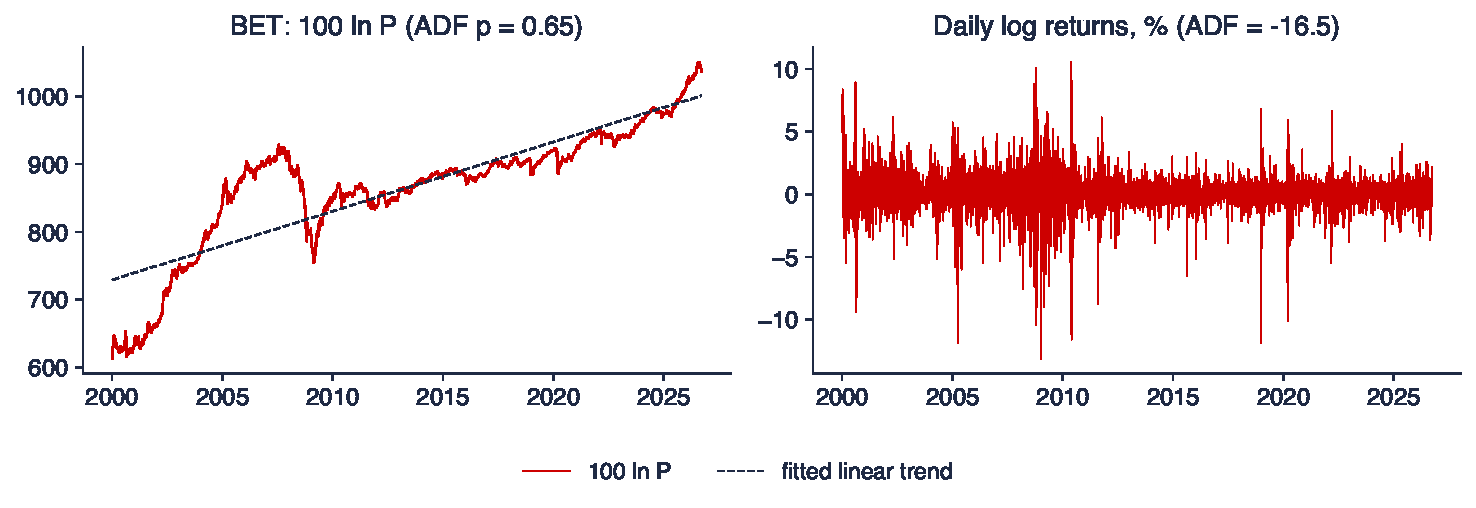
\includegraphics[width=0.96\textwidth,height=0.36\textheight,keepaspectratio]{ch3_sem_b1.pdf}
\end{center}
\vspace{-2mm}
\begin{center}
\scriptsize
\begin{tabular}{lrrrl}
\toprule
& ADF (p, $k$) & PP & KPSS & \textbf{verdict} \\
\midrule
$p_t$ (c, t) & $-1{,}90$ (0{,}653, 19) & $-2{,}35$ & 1{,}143 & $I(1)$ \\
$r_t$ (c) & $-16{,}50$ ($<$\,0{,}001, 18) & $-74{,}55$ & 0{,}360 & $I(0)$ \\
\bottomrule
\end{tabular}
\end{center}
\begin{itemize}
    \item $p_t$: ADF și PP mult peste $-3{,}41$, KPSS $> 0{,}146$: rădăcină unitară; $r_t$: ambele resping puternic, KPSS $< 0{,}463$: staționar
    \item Interpretare: nu; cu o rădăcină unitară, dreapta de trend nu atrage seria; la sfîrșitul eșantionului indicele se află la 39 puncte logaritmice de dreaptă și nimic nu îl readuce
\end{itemize}\quantlet{TSA\_ch3\_seminar}{\qlurl{TSA_ch3_seminar}}
\end{frame}

\begin{frame}{B2: S\&P 500 și EUR/RON [Propus]}
\itemsize{\footnotesize}
\begin{itemize}
\item \textbf{Întrebarea}: dau S\&P 500 și cursul EUR/RON aceleași verdicte ca BET?
\item \textbf{Date}: S\&P 500 din 2000; EUR/RON (cursul de referință BNR) din iulie 2005; ambele ca $100\ln$; model: B1
\item \textbf{Cerințe}
\begin{enumerate}
    \item Repetați pașii 2 și 3 din B1 pentru ambele serii.
    \item Comparați statisticile ADF și PP ale randamentelor și explicați de ce PP este mult mai negativ.
    \item Interpretare: cursul EUR/RON este administrat de banca centrală; spune rezultatul testului că el este un mers aleator?
\end{enumerate}
\item \textbf{Raportați}: un tabel (două serii, cîte două rînduri) și două fraze
\item Notebook: secțiunea B2
\end{itemize}
\end{frame}

\ifsolutions
\begin{frame}{B2: rezolvare [Propus]}
\itemsize{\scriptsize}
\begin{center}
\scriptsize
\begin{tabular}{lrrrl}
\toprule
& ADF (p, $k$) & PP & KPSS & \textbf{verdict} \\
\midrule
S\&P 500, $p_t$ (c, t) & $-2{,}08$ (0{,}557, 34) & $-2{,}36$ & 2{,}281 & $I(1)$ \\
S\&P 500, $r_t$ (c) & $-14{,}26$ ($<$\,0{,}001, 35) & $-91{,}41$ & 0{,}449 & $I(0)$ \\
EUR/RON, $s_t$ (c, t) & $-2{,}30$ (0{,}434, 7) & $-2{,}29$ & 1{,}431 & $I(1)$ \\
EUR/RON, $\Delta s_t$ (c) & $-27{,}42$ ($<$\,0{,}001, 6) & $-60{,}82$ & 0{,}055 & $I(0)$ \\
\bottomrule
\end{tabular}
\end{center}
\begin{itemize}
    \item Ambele niveluri: rădăcină unitară (ADF și PP nu resping, KPSS respinge); ambele serii de randamente: staționare
    \item PP nu folosește decalaje și corectează $\tau$ prin varianța pe termen lung; cu mii de observații ambele resping, PP mai puternic; verdictul este același
    \item Interpretare: nu; testele spun doar că seria nu revine la o medie sau la o dreaptă fixă; un curs administrat, cu ajustări mari și rare, poate arăta la fel (Cursul 3, Zivot--Andrews)
\end{itemize}\quantlet{TSA\_ch3\_seminar}{\qlurl{TSA_ch3_seminar}}
\end{frame}
\fi

\begin{frame}{B3: un model ARIMA pentru PIB-ul României [Rezolvat]}
\itemsize{\footnotesize}
\begin{itemize}
\item \textbf{Întrebarea}: ce model ARIMA descrie PIB-ul real al României și cît de incertă este o prognoză pe doi ani?
\item \textbf{Date}: PIB-ul real, volume înlănțuite (2010), ajustat sezonier, Eurostat, din T1 2000; $y_t = 100\ln Y_t$
\item \textbf{Cerințe}
\begin{enumerate}
    \item Alegeți $d$ cu ADF și KPSS pe $y_t$ (constantă și trend) și pe $\Delta y_t$ (constantă).
    \item Estimați ARIMA$(p,1,q)$ cu derivă pentru $p, q \le 2$ și alegeți modelul cu cel mai mic AICc.
    \item Verificați reziduurile cu Ljung--Box $Q^*(8)$.
    \item Prognozați 8 trimestre, cu intervale de 80\% și 95\%.
    \item Interpretare: de ce este intervalul de 95\% după 8 trimestre de aproximativ două ori mai larg decît după 2 trimestre?
\end{enumerate}
\item \textbf{Raportați}: testele, AICc pentru șase modele, modelul ales, $Q^*(8)$, graficul și o frază
\item Notebook: secțiunea B3
\end{itemize}
\end{frame}

\begin{frame}{B3: rezolvare [Rezolvat]}
\itemsize{\scriptsize}
\begin{center}
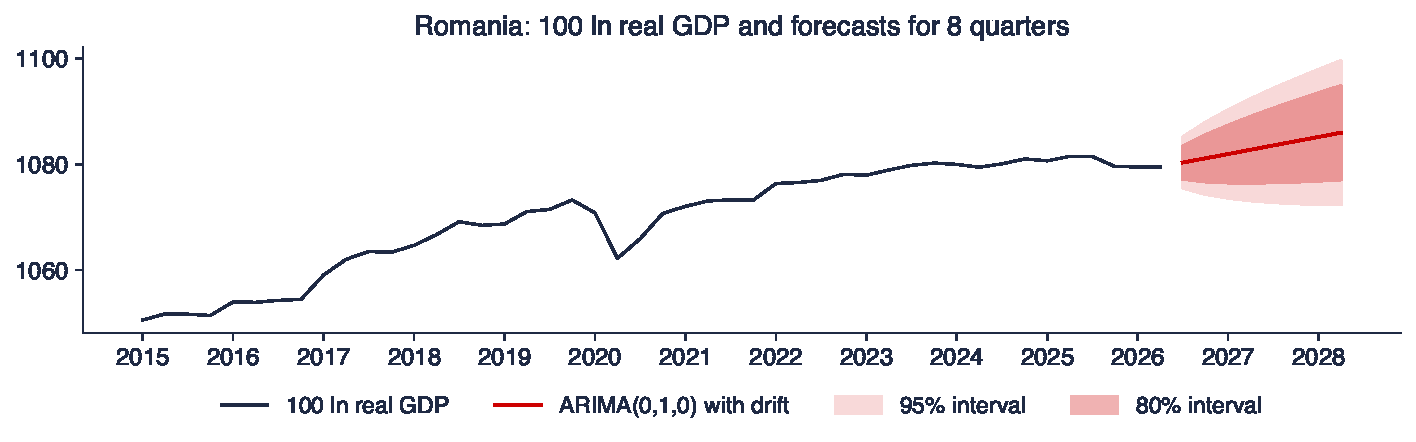
\includegraphics[width=0.96\textwidth,height=0.34\textheight,keepaspectratio]{ch3_sem_b3.pdf}
\end{center}
\vspace{-2mm}
\begin{itemize}
    \item $y_t$: ADF $-2{,}31$ (p = 0{,}428), KPSS 0{,}198 $> 0{,}146$: $I(1)$; $\Delta y_t$: ADF $-10{,}77$, KPSS 0{,}263: $I(0)$; deci $d = 1$
    \item AICc: (0,1,0) 491{,}9; (1,1,0) 493{,}8; (0,1,1) 493{,}7; (1,1,1) 494{,}9; (2,1,0) 493{,}7; (0,1,2) 493{,}6: ARIMA(0,1,0) cu deriva $\hat c = 0{,}81$ (SE 0{,}30), $\hat\sigma = 2{,}47$
    \item $Q^*(8) = 7{,}3$ (p = 0{,}51): reziduuri de tip zgomot alb; prognoza pentru T2 2028: 1086{,}0, adică $+6{,}5$\% în doi ani, intervalul de 95\% $[1072{,}3; 1099{,}7]$
    \item Interpretare: pentru un mers aleator varianța erorii este $h\sigma^2$, deci lățimea crește ca $\sqrt{h}$: $\sqrt{8/2} = 2$ (semilățimile 6{,}8 și 13{,}7, raportul 2{,}00)
\end{itemize}\quantlet{TSA\_ch3\_seminar}{\qlurl{TSA_ch3_seminar}}
\end{frame}

\begin{frame}{B4: inflația din România, $d = 0$ sau $d = 1$? [Propus]}
\itemsize{\footnotesize}
\begin{itemize}
\item \textbf{Întrebarea}: este inflația anuală din România staționară și cît de mult schimbă răspunsul prognoza?
\item \textbf{Date}: $\pi_t = 100(\ln P_t - \ln P_{t-12})$, IAPC, ianuarie 2005--august 2026; model: B3
\item \textbf{Cerințe}
\begin{enumerate}
    \item Aplicați ADF, PP și KPSS pe $\pi_t$ și pe $\Delta\pi_t$, cu constantă.
    \item Găsiți cel mai bun ARIMA$(p,0,q)$ cu medie și cel mai bun ARIMA$(p,1,q)$ după AICc, cu $p \le 3$, $q \le 2$.
    \item Prognozați 12 luni cu ambele modele, cu intervale de 95\%, și aplicați Ljung--Box $Q^*(24)$ pe reziduurile lor.
    \item Interpretare: de ce dau cele două modele prognoze punctuale similare, dar intervale diferite?
\end{enumerate}
\item \textbf{Raportați}: un tabel cu testele, două modele, două prognoze cu intervale, două teste Ljung--Box și două fraze
\item Notebook: secțiunea B4
\end{itemize}
\end{frame}

\ifsolutions
\begin{frame}{B4: rezolvare [Propus]}
\itemsize{\scriptsize}
\begin{center}
\includegraphics[width=0.96\textwidth,height=0.34\textheight,keepaspectratio]{ch3_sem_b4.pdf}
\end{center}
\vspace{-2mm}
\begin{itemize}
    \item $\pi_t$: ADF $-1{,}94$ (p = 0{,}315), KPSS 0{,}404 $< 0{,}463$: neconcludent; $\Delta\pi_t$: ADF $-4{,}83$, KPSS 0{,}105: $I(0)$
    \item $d = 0$: ARIMA(2,0,0), suma coeficienților AR 0{,}976, media 5{,}2\%; 12 luni: 5{,}1\% în $[0{,}3; 9{,}9]$. $d = 1$: ARIMA(1,1,0); 5{,}2\% în $[-0{,}4; 10{,}8]$
    \item $Q^*(24)$: 71 (p $<$\,0{,}001) și 97 (p $<$\,0{,}001): ambele lasă autocorelație, deoarece ratele anuale se suprapun (\tsachlink{https://danpele.github.io/Time-Series-Analysis/RO/Cursuri/capitol4_sezonalitate_prognoza.pdf}{Capitolul 4} modelează inflația lunară)
    \item Interpretare: suma coeficienților AR, 0{,}976, este aproape 1, deci pe termen scurt modelele evoluează la fel; doar $d = 1$ lasă varianța erorii să crească nelimitat, de aici intervalul mai larg
\end{itemize}\quantlet{TSA\_ch3\_seminar}{\qlurl{TSA_ch3_seminar}}
\end{frame}
\fi


%=============================================================================
\section{Partea C: întrebări deschise și critica unui răspuns AI}
%=============================================================================

\begin{frame}{C1: ruptură sau rădăcină unitară? [Propus]}
\itemsize{\footnotesize}
\begin{itemize}
\item \textbf{Întrebarea}: au inflația și PIB-ul României o rădăcină unitară sau sînt staționare în jurul unei medii ori al unui trend care s-a schimbat o dată?
\item \textbf{Date}: $\pi_t$ din B4 și $y_t$ din B3; modele: B1, B3
\item \textbf{Cerințe}
\begin{enumerate}
    \item Aplicați testul Zivot--Andrews cu ruptură în nivel, apoi în nivel și în trend, pe ambele serii.
    \item Comparați fiecare statistică cu valoarea critică de 5\% și raportați datele rupturilor.
    \item Asociați datele cu evenimente (țintirea inflației din 2005, criza din 2008--2009, șocul energetic din 2022).
    \item Interpretare: de ce trebuie comparată cu istoria o dată de ruptură găsită de un test înainte de a o accepta?
\end{enumerate}
\item \textbf{Raportați}: un tabel cu patru statistici și datele lor, graficul și un plan de proiect
\item Notebook: secțiunea C1
\end{itemize}
\end{frame}

\ifsolutions
\begin{frame}{C1: analiză de referință [Propus]}
\itemsize{\scriptsize}
\begin{center}
\includegraphics[width=0.96\textwidth,height=0.34\textheight,keepaspectratio]{ch3_sem_c1.pdf}
\end{center}
\vspace{-2mm}
\begin{itemize}
    \item Inflația: ZA (nivel) $= -3{,}65$ (p = 0{,}58), peste $-4{,}81$, ruptură în aprilie 2021: nicio dovadă împotriva rădăcinii unitare
    \item PIB: ZA (nivel) $= -3{,}73$, nesemnificativ; ZA (nivel și trend) $= -5{,}27$ $< -5{,}07$ (p = 0{,}028), ruptură în T4 2008: staționar în jurul unui trend care s-a rupt în criza din 2008?
    \item Interpretare: testul alege data care se potrivește cel mai bine datelor; o dată fără un eveniment economic sau găsită după încercarea mai multor specificații poate fi un accident al eșantionului
    \item Proiect: rupturi și persistența inflației în România și în regiune, cu testul Bai--Perron pentru mai multe rupturi
\end{itemize}\quantlet{TSA\_ch3\_seminar}{\qlurl{TSA_ch3_seminar}}
\end{frame}
\fi

\begin{frame}{C2: verificați un răspuns AI [Propus]}
\itemsize{\scriptsize}
\begin{itemize}
    \item Un student a cerut unui asistent AI să analizeze PIB-ul și prețurile din România. Răspunsul:
    \item \aiprompt{(a) Valoarea p ADF pentru logaritmul PIB este 0{,}43, deci s-a demonstrat că PIB-ul are rădăcină unitară.}
    \item \aiprompt{(b) Statistica KPSS pentru logaritmul PIB este 0{,}198, peste 0,146, deci KPSS respinge rădăcina unitară.}
    \item \aiprompt{(c) Regresia logaritmului IAPC pe logaritmul S\&P 500 dă t = 34{,}6 și R2 = 0{,}82: acțiunile americane determină prețurile din România.}
    \item \aiprompt{(d) Creșterea PIB este staționară, deci încă o diferențiere va face modelul ARIMA și mai bun.}
    \item \aiprompt{(e) O prognoză de tip mers aleator are aceeași lățime a intervalului de 95\% la orice orizont.}
    \item \aiprompt{(f) Valoarea critică Dickey-Fuller de 5\% cu constantă este circa -2{,}87, mai negativă decît -1,645, pentru că distribuția Dickey-Fuller este deplasată la stînga.}
    \item Cerințe
    \begin{itemize}
        \item 1. Pentru fiecare afirmație, precizați dacă este corectă; dacă nu este, formulați afirmația corectă și, acolo unde se poate, dați valoarea corectă din notebook (secțiunea C2).
        \item 2. Raportați: o listă de șase verdicte, fiecare cu un rînd de justificare.
    \end{itemize}
\end{itemize}
\end{frame}

\ifsolutions
\begin{frame}{C2: rezolvare [Propus]}
\itemsize{\scriptsize}
\begin{itemize}
    \item (a) Greșit: nerespingerea nu este o demonstrație; cu 106 trimestre testul are putere mică împotriva unui $\phi$ apropiat de 1
    \item (b) Greșit: ipoteza nulă KPSS este staționaritatea; 0{,}198 $> 0{,}146$ respinge staționaritatea, ceea ce susține rădăcina unitară
    \item (c) Greșit: o regresie falsă între două serii cu trend; DW = 0{,}03 $< R^2$; în diferențe $t = -0{,}21$
    \item (d) Greșit: supradiferențiere; rădăcina MA ajunge pe cercul unitate, iar varianța crește
    \item (e) Greșit: varianța este $h\sigma^2$, deci lățimea crește ca $\sqrt{h}$
    \item (f) Corect
\end{itemize}\quantlet{TSA\_ch3\_seminar}{\qlurl{TSA_ch3_seminar}}
\end{frame}
\fi


%=============================================================================
\section{Încheiere}
%=============================================================================

\begin{frame}{Idei de reținut}
\itemsize{\small}
\begin{itemize}
    \item Comparați $\tau$ cu valorile critice Dickey--Fuller, niciodată cu cele ale distribuției Normale; alegeți termenii determiniști după grafic
    \item ADF și KPSS au ipoteze nule opuse: interpretați-le împreună
    \item Prețurile, cursurile de schimb și PIB-ul în logaritmi sînt $I(1)$; randamentele și ratele de creștere sînt $I(0)$
    \item Cu $d = 1$, intervalele de prognoză cresc cu orizontul; alegerea lui $d$ contează mai ales pe orizonturi lungi
    \item Un răspuns AI este o ciornă: verificați sensul fiecărui test și valorile critice folosite
\end{itemize}
\end{frame}

\begin{frame}{După seminar}
\itemsize{\small}
\begin{itemize}
    \item Cursul 3 dezvoltă fiecare temă de azi: trendurile, regresia falsă, distribuțiile Dickey--Fuller, PP, KPSS, rupturile, prognoza ARIMA și selecția automată
    \item Încercați cerințele [Propus] în notebook
    \item C1 poate deveni un proiect de echipă: rupturi și persistența inflației în România, Ungaria, Polonia și Cehia
    \item Lectură: \refHP, cap.~4--5; \refFPP, cap.~9; \refHamilton, cap.~15--17
    \item \textbf{Seminarul are rol de exercițiu și nu se notează; rezolvările cerințelor [Propus] se discută la seminar}
\end{itemize}
\end{frame}


%=============================================================================
\section{Bibliografie}
%=============================================================================

\begin{frame}{Bibliografie}
\itemsize{\tiny}
\begin{itemize}
    \item Dickey, D. A., \& Fuller, W. A. (1979). Distribution of the estimators for autoregressive time series with a unit root. \textit{Journal of the American Statistical Association}, 74(366), 427--431. \href{https://doi.org/10.1080/01621459.1979.10482531}{doi:10.1080/01621459.1979.10482531}
    \item Granger, C. W. J., \& Newbold, P. (1974). Spurious regressions in econometrics. \textit{Journal of Econometrics}, 2(2), 111--120. \href{https://doi.org/10.1016/0304-4076(74)90034-7}{doi:10.1016/0304-4076(74)90034-7}
    \item Hamilton, J. D. (1994). \textit{Time Series Analysis}. Princeton University Press. \href{https://doi.org/10.2307/j.ctv14jx6sm}{doi:10.2307/j.ctv14jx6sm}
    \item Huang, C., \& Petukhina, A. (2022). \textit{Applied Time Series Analysis and Forecasting with Python}. Springer. \href{https://doi.org/10.1007/978-3-031-13584-2}{doi:10.1007/978-3-031-13584-2}
    \item Hyndman, R. J., \& Athanasopoulos, G. (2021). \textit{Forecasting: Principles and Practice} (3rd ed.). OTexts. \href{https://otexts.com/fpp3/}{otexts.com/fpp3}
    \item Kwiatkowski, D., Phillips, P. C. B., Schmidt, P., \& Shin, Y. (1992). Testing the null hypothesis of stationarity against the alternative of a unit root. \textit{Journal of Econometrics}, 54(1--3), 159--178. \href{https://doi.org/10.1016/0304-4076(92)90104-Y}{doi:10.1016/0304-4076(92)90104-Y}
    \item MacKinnon, J. G. (1994). Approximate asymptotic distribution functions for unit-root and cointegration tests. \textit{Journal of Business \& Economic Statistics}, 12(2), 167--176. \href{https://doi.org/10.1080/07350015.1994.10510005}{doi:10.1080/07350015.1994.10510005}
    \item MacKinnon, J. G. (2010). Critical values for cointegration tests. Queen's Economics Department Working Paper No.~1227, Queen's University. \href{https://ideas.repec.org/p/qed/wpaper/1227.html}{ideas.repec.org/p/qed/wpaper/1227}
    \item Phillips, P. C. B., \& Perron, P. (1988). Testing for a unit root in time series regression. \textit{Biometrika}, 75(2), 335--346. \href{https://doi.org/10.1093/biomet/75.2.335}{doi:10.1093/biomet/75.2.335}
    \item Zivot, E., \& Andrews, D. W. K. (1992). Further evidence on the Great Crash, the oil-price shock, and the unit-root hypothesis. \textit{Journal of Business \& Economic Statistics}, 10(3), 251--270. \href{https://doi.org/10.1080/07350015.1992.10509904}{doi:10.1080/07350015.1992.10509904}
\end{itemize}
\end{frame}

\end{document}
